\documentclass{article}

% if you need to pass options to natbib, use, e.g.:
\PassOptionsToPackage{numbers, compress}{natbib}
% before loading nips_2016
%
% to avoid loading the natbib package, add option nonatbib:
% \usepackage[nonatbib]{nips_2016}

% \usepackage{nips_2016}
% \usepackage[nonatbib]{nips_2016}

% to compile a camera-ready version, add the [final] option, e.g.:
\usepackage[final]{nips_2016}

\usepackage[utf8]{inputenc} % allow utf-8 input
\usepackage[T1]{fontenc}    % use 8-bit T1 fonts
\usepackage{url}            % simple URL typesetting
\usepackage{booktabs}       % professional-quality tables
\usepackage{amsfonts}       % blackboard math symbols
\usepackage{hyperref}
\usepackage{amsmath}        % math package
\usepackage{nicefrac}       % compact symbols for 1/2, etc.
\usepackage{graphicx}       % compact symbols for 1/2, etc.
\usepackage{microtype}      % microtypography
\usepackage{subfig}      % multiple captions and labels in a single figure
\usepackage{amsmath}
\usepackage[font={footnotesize}]{caption}
\usepackage{enumitem}

\usepackage{rotating}
\usepackage{array}

\setlist{nosep}


\usepackage{color}
\newcommand{\razp}[1]{\textcolor{blue}{#1}}

\title{Progressive Neural Networks}


\author{Andrei A. Rusu*, \ Neil C. Rabinowitz*, \ Guillaume Desjardins*, \ Hubert Soyer,\\
\textbf{James Kirkpatrick, \ Koray Kavukcuoglu, \ Razvan Pascanu, \ Raia Hadsell} \\
\small{* These authors contributed equally to this work}
\vspace{0.15 cm}
\\
Google DeepMind \\
London, UK
\vspace{0.15 cm}
\\
\small\texttt{\{andreirusu, ncr, gdesjardins, soyer, kirkpatrick, korayk, razp, raia\}@google.com} \\
}
\begin{document}
% \nipsfinalcopy is no longer used

\maketitle

\begin{abstract}
Learning to solve complex sequences of tasks---while both leveraging transfer and
avoiding catastrophic forgetting---remains a key obstacle to achieving human-level
intelligence. The \emph{progressive networks} approach represents a step forward in this direction:
they are immune to forgetting and can leverage prior knowledge via lateral
connections to previously learned features. We evaluate this architecture
extensively on a wide variety of reinforcement learning tasks (Atari and 3D
maze games), and show that it outperforms common baselines based on pretraining
and finetuning. Using a novel sensitivity measure, we demonstrate
that transfer occurs at both low-level sensory and high-level control layers of the learned policy.
\end{abstract}

version https://git-lfs.github.com/spec/v1
oid sha256:f7f279fa0f93cb2842457a52f2e0361e29261eb78732a2e3ff4c6aebddfefb19
size 6684

\section{Progressive Networks}

Continual learning is a long-standing goal of machine learning, where agents
not only learn (and remember) a series of tasks experienced in sequence, but also have
the ability to transfer knowledge from previous tasks to improve convergence speed \cite{AAAIMag11-Taylor}.
\textit{Progressive networks} integrate these desiderata directly into the
model architecture: catastrophic forgetting is prevented by instantiating a new
neural network (a \textit{column}) for each task being solved, while transfer is
enabled via lateral connections to features of previously learned columns. The
scalability of this approach is addressed at the end of this section.

A progressive network starts with a single column: a deep neural network having
$L$ layers with hidden activations $h_i^{(1)} \in \mathbb{R}^{n_i}$,
with $n_i$ the number of units at layer $i \le L$, and parameters
$\Theta^{(1)}$ trained to convergence.  When switching to a second task, the
parameters $\Theta^{(1)}$ are ``frozen'' and a new
column with parameters $\Theta^{(2)}$ is instantiated (with random
initialization), where layer $h_i^{(2)}$ receives input from both
$h_{i-1}^{(2)}$ and $h_{i-1}^{(1)}$ via lateral connections. This
generalizes to $K$ tasks as follows:
\footnote{Progressive networks can also be generalized in a straightforward
manner to have arbitrary network width per column/layer, to accommodate varying
degrees of task difficulty, or to compile lateral connections from multiple,
independent networks in an ensemble setting. Biases are omitted for clarity.}:
\begin{align}
  \label{eq:prognet}
  h_i^{(k)} = f\left( W_i^{(k)} h_{i-1}^{(k)} + \sum_{j<k} U_{i}^{(k:j)} h_{i-1}^{(j)} \right),
\end{align}
where $W_i^{(k)} \in \mathbb{R}^{n_{i} \times n_{i-1}}$ is the weight matrix of layer
$i$ of column $k$, $U_{i}^{(k:j)} \in \mathbb{R}^{n_i \times n_j}$ are the
lateral connections from layer $i-1$ of column $j$, to layer $i$ of column $k$
and $h_0$ is the network input.
$f$ is an element-wise non-linearity: we use $f(x)=\max(0, x)$ for all
intermediate layers.
A progressive network with $K=3$ is shown in Figure~\ref{fig:progressiveNet}.

\begin{figure}[h]
  \centering
    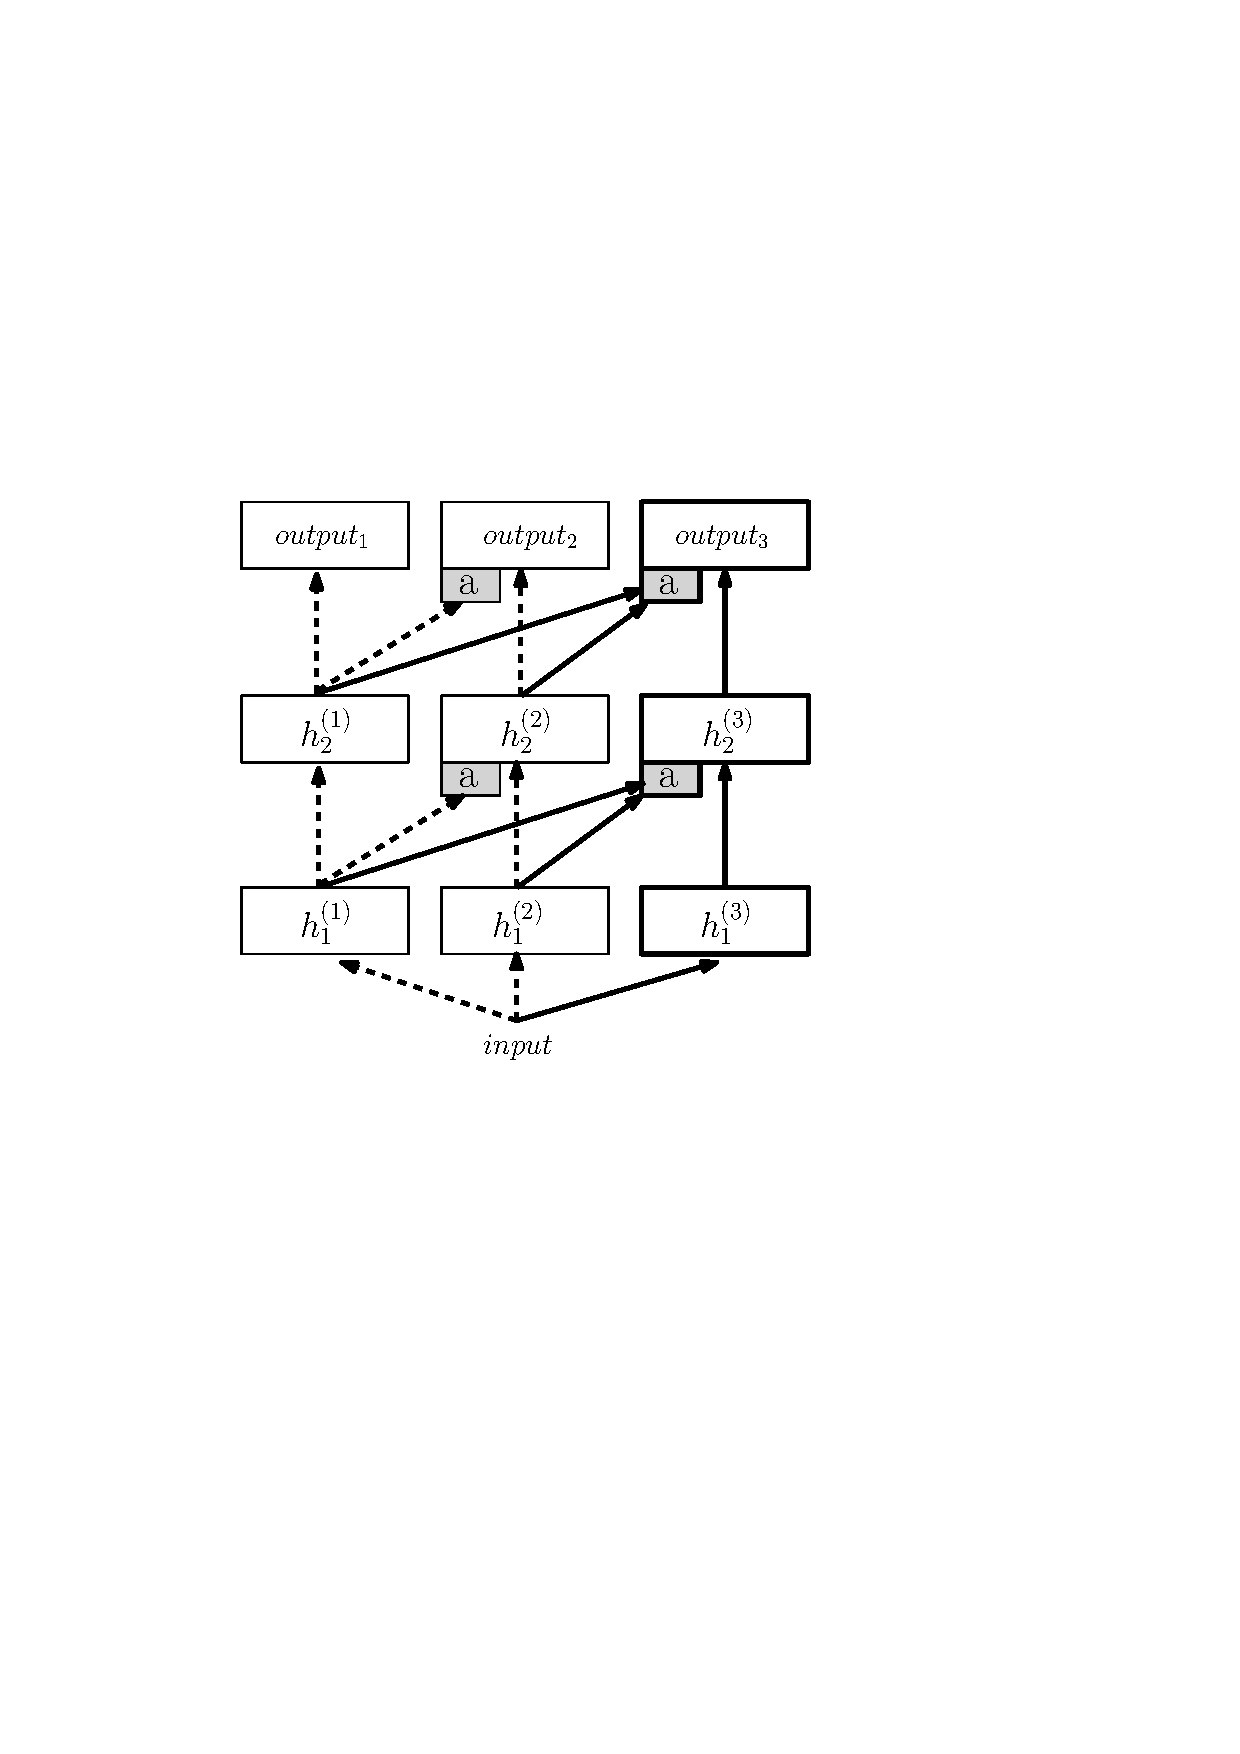
\includegraphics[width=.25\textwidth]{figures/progressiveNetDepiction2}
    \caption{Depiction of a three column progressive network. The first two
columns on the left (dashed arrows) were trained on task 1 and 2 respectively.
The grey box labelled $a$ represent the adapter layers (see text).
A third column is added for the final task having access to all previously learned
features.
    }
    \label{fig:progressiveNet}
\end{figure}

These modelling decisions are informed by our desire to:
(1) solve $K$ independent tasks at the end of training;
(2) accelerate learning via transfer when possible; and
(3) avoid catastrophic forgetting.

In the standard pretrain-and-finetune paradigm, there is often an implicit
assumption of ``overlap'' between the tasks. Finetuning is efficient in this
setting, as parameters need only be adjusted slightly to
the target domain, and often only the top layer is retrained \cite{yosinski-nips2014}. In contrast, we make no assumptions about the
relationship between tasks, which may in practice be orthogonal or even
adversarial. While the finetuning stage could potentially unlearn these
features, this may prove difficult. Progressive networks side-step
this issue by allocating a new column for each new task, whose weights are
initialized randomly. Compared to the task-relevant initialization of pretraining,
columns in progressive networks are free to reuse, modify or ignore previously
learned features via the lateral connections.
As the lateral connections $U_{i}^{(k:j)}$ are only from column $k$ to columns
$j < k$, previous columns are not affected by the newly learned features in the
forward pass.  Because also the parameters $\{ \Theta^{(j)}; j<k\}$
are kept frozen (i.e. are constants for the optimizer) when training $\Theta^{(k)}$,
there is no interference between
tasks and hence no catastrophic forgetting.

\paragraph{Application to Reinforcement Learning.} Although progressive
networks are widely applicable, this paper focuses on their application to
deep reinforcement learning. In this case, each column is trained to solve a
particular Markov Decision Process (MDP): the $k$-th column thus defines a policy
$\pi^{(k)}(a\mid s)$ taking as input a state $s$ given by the environment,
and generating probabilities over actions $\pi^{(k)}(a\mid s) := h_L^{(k)}(s)$.
At each time-step, an action is sampled from this distribution and taken in the
environment, yielding the subsequent state. This policy implicitly defines a
stationary distribution $\rho_{\pi^{(k)}}(s,a)$ over states and actions.

\paragraph{Adapters.}
In practice, we augment the progressive network layer of Equation~\ref{eq:prognet} with
non-linear lateral connections which we call \textit{adapters}. They serve
both to improve initial conditioning and perform dimensionality reduction.
Defining the vector of anterior features
$h_{i-1}^{(<k)} = [h_{i-1}^{(1)} \cdots h_{i-1}^{(j)} \cdots h_{i-1}^{(k-1)}]$
of dimensionality $n_{i-1}^{(<k)}$, in the case of dense layers,
we replace the linear lateral connection with a single hidden layer MLP.
Before feeding the lateral activations into the MLP, we multiply them by a learned scalar,
initialized by a random small value.
Its role is to adjust for the different scales of the different inputs.
The hidden layer of the non-linear adapter is a projection onto an $n_{i}$ dimensional
subspace.  As the
index $k$ grows, this ensures that the number of parameters stemming from the
lateral connections is in the same order as $\left|\Theta^{(1)} \right|$. Omitting bias
terms, we get:
\begin{align}
  \label{eq:prognet}
  h_i^{(k)} = \sigma \left( W_i^{(k)} h_{i-1}^{(k)} + U_{i}^{(k:j)} \sigma(V_{i}^{(k:j)} \alpha_{i-1}^{(<k)} h_{i-1}^{(<k)}) \right),
\end{align}
where $V_{i}^{(k:j)} \in \mathbb{R}^{n_{i-1} \times n_{i-1}^{(<k)}}$ is the projection
matrix. For convolutional layers, dimensionality reduction is
performed via $1\times 1$ convolutions \cite{LinCY13}.

\paragraph{Limitations.}
\textit{Progressive networks} are a stepping stone towards a full continual
learning agent: they contain the necessary ingredients to learn multiple tasks,
in sequence, while enabling transfer and being immune to catastrophic
forgetting. A downside of the approach is the growth in number of
parameters with the number of tasks.
The analysis of Appendix 2 reveals
that only a fraction of the new capacity is actually utilized, and that this trend increases with more columns. This
suggests that growth can be addressed, e.g. by adding fewer layers or less capacity, by pruning \cite{Cun90optimalbrain}, or by online compression
\cite{Rusu15} during learning.  Furthermore, while progressive networks retain the
ability to solve all $K$ tasks at test time, choosing which column to use for
inference requires knowledge of the task label. These issues are left as future
work.

\section{Transfer Analysis}
\label{sec_transfer}

Unlike finetuning, progressive nets do not destroy the features learned on
prior tasks. This enables us to study in detail which features and at which
depth transfer actually occurs. We explored two related methods: an intuitive,
but slow method based on a perturbation analysis, and a faster analytical method
derived from the Fisher Information \cite{amari98natural}.

\paragraph{Average Perturbation Sensitivity (APS).} To evaluate the degree to
which source columns contribute to the target task, we can inject
Gaussian noise at isolated points in the architecture (e.g. a given
layer of a single column) and measure the impact of this perturbation
on performance. A significant drop in performance indicates that the
final prediction is heavily reliant on the feature map or
layer. We find that this method yields similar results to the faster
Fisher-based method presented below. We thus relegate details and
results of the perturbation analysis to the appendix.

\paragraph{Average Fisher Sensitivity (AFS).}
We can get a local approximation to the perturbation sensitivity by using
the Fisher Information matrix
\cite{amari98natural}. While the Fisher matrix is typically computed with
respect to the model
parameters, we compute a modified diagonal Fisher $\hat{F}$ of the network policy $\pi$
with respect to the \textit{normalized activations}
\footnote{The Fisher of individual neurons (fully connected) and feature maps
(convolutional layers) are computed over $\rho_{\pi^{(k)}}(s,a)$. The use of a normalized
representation $\hat{h}$ is non-standard, but makes the scale of $\hat{F}$
comparable across layers and columns.}
at each layer $\hat{h}_i^{(k)}$. For convolutional layers, we define
$\hat{F}$ to implicitly perform a summation over pixel locations. $\hat{F}$ can
be interpreted as the sensitivity of the policy to small changes in the
representation. We define the diagonal matrix $\hat{F}$, having
elements $\hat{F}(m,m)$, and the derived Average Fisher
Sensitivity (AFS) of feature $m$ in layer $i$ of column $k$ as:
\begin{align*}
\hat{F}_i^{(k)} &=
     \mathbb{E}_{\rho(s, a)}
        \left[
          \frac {\partial \log \pi} {\partial \hat{h}_i^{(k)}} \,
          \frac {\partial \log \pi} {\partial \hat{h}_i^{(k)}}^T
        \right]
& \hspace{1cm} &
\text{AFS}(i,k,m) &=
    \frac{\hat{F}_i^{(k)}(m,m)}{\sum_k \hat{F}_i^{(k)}(m,m)}
\end{align*}
where the expectation is over the joint state-action distribution $\rho(s,a)$
induced by the progressive network
trained on the target task. In practice, it is often useful to consider the AFS
score per-layer $\text{AFS}(i,k) = \sum_m \text{AFS}(i,k,m)$, i.e. summing over
all features of layer $i$. The AFS and APS thus estimate how much
the network relies on each feature or column in a layer to compute its output.

version https://git-lfs.github.com/spec/v1
oid sha256:ac4d7ee4654fc3ffca23ee016831c5e8f4efff208f631ba4b5484e8413aca25e
size 4146

\newpage
\section{Detailed Experiment Setup}
\label{sec:appendix_exp_setup}
\subsection{Datasets}
\label{sec:appendix_exp_dataset}
We conduct experiment on CIFAR-10, CIFAR-100 (MIT) \citep{Krizhevsky09learningmultiple} (\url{https://www.cs.toronto.edu/~kriz/cifar.html}), and MNIST (CC BY-SA 3.0) \citep{lecun1998gradient} (\url{http://yann.lecun.com/exdb/mnist/}). The datasets are downloaded through torchvision \citep{NEURIPS2019_9015} (\url{https://pytorch.org/vision/stable/index.html}). We used their default splitting of training and testing set.

To compare our work on PAC-Bayes bound with the work of \citet{dziugaite2017computing}, we created a custom dataset MNIST-2 by setting the label of images 0-4 to 0 and 5-9 to 1.
We also created random-labeled datasets MNIST-R and CIFAR10-R by randomly labeling the images from the training set of MNIST and CIFAR10.
The dataset information is summarized in \tableref{tab:appendix_dataset}
\begin{table}[h]
\small
  \centering
  \caption{Datasets}
  \vskip 0.1in
    \begin{center}

    \begin{tabular}{lccccc}
    \toprule
    &   \multicolumn{2}{c}{\# Data Points}    &    & &     \\
    Dataset & Train & Test & Input Size & \# Classes & Label \\
    \midrule
    CIFAR10 & 50000 & 10000 & $3\times32\times32$ & 10 & True \\
    CIFAR10-R & 50000 & 10000 & $3\times32\times32$ & 10 & Random \\
    CIFAR100 & 50000 & 10000 & $3\times32\times32$ & 100 & True \\
    MNIST & 60000 & 10000 & $28\times28$ & 10 & True \\
    MNIST-2 & 60000 & 10000 & $28\times28$ & 2 & True \\
    MNIST-R & 60000 & 10000 & $28\times28$ & 10 & Random \\\bottomrule
    \end{tabular}
\end{center}
  \label{tab:appendix_dataset}%
\end{table}%

All the datasets (MNIST, CIFAR-10, and CIFAR-100) we used are publicly available. According to their descriptions on the contents and collection methods, they should not contain any personal information or offensive content. MNIST is a remix of datasets from the National Institute of Standards and Technology (NIST), which obtained consent for collecting the data. However, we also note that CIFAR-10 and CIFAR-100 are subsets of the dataset 80 Million Tiny Image \citep{torralba2007tiny} (\url{http://groups.csail.mit.edu/vision/TinyImages/}), which used automatic collection and includes some offensive images.

\subsection{Network Structures}
\label{appendix_exp_nn}
\paragraph{Fully Connected Network:}
We used several different fully connected networks varying in the number of hidden layers and the number of neurons for each hidden layer. The output of all layers except the last layer are passed into ReLU before feeding into the subsequent layer.  As described in \sectionref{subsec:approx}, we denote a fully connected network with $m$ hidden layers and $n$ neurons each hidden layer by F-$n^m$. For networks without uniform layer width, we denote them by a sequence of numbers (e.g. for a network with three hidden layers, where the first two layers has 200 neurons each and the third has 100 neurons, we denote it as F-$200^2$-$100$). For example, the structure of F-$200^2$ is shown in \tableref{tab:appendix_fc_struct}.

\begin{table}[h]
\small
  \centering
  \caption{Structure of F-$200^2$ on MNIST}
  \vskip 0.1in
    \begin{center}
    \begin{tabular}{rllcc}
    \toprule
    \# & Name & Module & In Shape & Out Shape\\
    \midrule
    1 & & Flatten & (28,28) & 784\\
    2 & fc1 & Linear(784, 200) & 784 & 200\\
    3 & & ReLU & 200 & 200\\
    4 & fc2 & Linear(200, 200) & 200 & 200\\
    5 & & ReLU & 200 & 200\\
    6 & fc3 & Linear(200, 10) & 200 & 10\\
    \multicolumn{5}{c}{\emph{output}}\\\bottomrule
    \end{tabular}%
\end{center}

  \label{tab:appendix_fc_struct}%
\end{table}%

\paragraph{LeNet5:} We adopted the LeNet5 structure proposed by \citet{lecun1998gradient} for MNIST, and slightly modified the input convolutional layers to adapt the input of CIFAR-10 dataset. The standard LeNet5 structure we used in the experiments is shown in \tableref{tab:appendix_lenet_struct}. We further modified the dimension of fc1 and conv2 to create several variants for the experiment in \sectionref{sec:models}. Take the model whose first fully connected layer is adjusted to have 80 neurons as an example, we denote it as LeNet5-(fc1-80).

\begin{table}[h]
\small
  \centering
  \caption{Structure of LeNet5 on CIFAR-10}
  \vskip 0.1in
    \begin{center}
    \begin{tabular}{rllcc}
    \toprule
    \# & Name & Module & In Shape & Out Shape\\\midrule
    1 & conv1 & Conv2D(3, 6, 5, 5) & (3, 32, 32) & (6, 28, 28)\\
    2 & & ReLU & (6, 28, 28) & (6, 28, 28)\\
    3 & maxpool1 & MaxPooling2D(2,2) & (6, 28, 28) & (6, 14, 14)\\
    4 & conv2 & Conv2D(6, 16, 5, 5) & (6, 14, 14) & (16, 10, 10)\\
    5 & & ReLU & (16, 10, 10) & (16, 10, 10)\\
    6 & maxpool2 & MaxPooling2D(2,2) & (16, 10, 10) & (16, 5, 5)\\
    7 & & Flatten & (16, 5, 5) & 400\\
    8 & fc1 & Linear(400, 120) & 400 & 120\\
    9 & & ReLU & 120 & 120\\
    10 & fc2 & Linear(120, 84) & 120 & 84\\
    11 & & ReLU & 84 & 84\\
    12 & fc3 & Linear(84, 10) & 84 & 10\\
    \multicolumn{5}{c}{\emph{output}} \\\bottomrule
    \end{tabular}%
\end{center}
  \label{tab:appendix_lenet_struct}%
\end{table}%

\paragraph{Networks with Batch Normalization:} In \sectionref{sec:appendix_batchnorm} we conducted several experiments regarding the effect of batch normalization on our results. For those experiments, we use the existing structures and add batch normalization layer for each intermediate output after it passes the ReLU module. In order for the Hessian to be well-defined, we fix the running statistics of batch normalization and treat it as a linear layer during inference. We also turn off the learnable parameters $\theta$ and $\beta$ \citep{ioffe2015batch} for simplicity. For network structure X, we denote the variant with batch normalization after all hidden layers X-BN.
For example, the detailed structure LeNet5-BN is shown in \tableref{tab:appendix_lenetBN_struct}.

\begin{table}[h]
\small
  \centering
  \caption{Structure of LeNet5-BN on CIFAR-10}
  \vskip 0.1in
  \begin{center}
    \begin{tabular}{rllcc}
    \toprule
    \# & Name & Module & In Shape & Out Shape\\\midrule
    1 & conv1 & Conv2D(3, 6, 5, 5) & (3, 32, 32) & (6, 28, 28)\\
    2 & & ReLU & (6, 28, 28) & (6, 28, 28)\\
    3 & & BatchNorm2D & (6, 28, 28) & (6, 28, 28)\\
    4 & maxpool1 & MaxPooling2D(2,2) & (6, 28, 28) & (6, 14, 14)\\
    5 & conv2 & Conv2D(6, 16, 5, 5) & (6, 14, 14) & (16, 10, 10)\\
    6 & & ReLU & (16, 10, 10) & (16, 10, 10)\\
    7 & & BatchNorm2D & (16, 10, 10) & (16, 10, 10)\\
    8 & maxpool2 & MaxPooling2D(2,2) & (16, 10, 10) & (16, 5, 5)\\
    9 & & Flatten & (16, 5, 5) & 400\\
    10 & fc1 & Linear(400, 120) & 400 & 120\\
    11 & & ReLU & 120 & 120\\
    12 & & BatchNorm1D & 120 & 120\\
    13 & fc2 & Linear(120, 84) & 120 & 84\\
    14 & & ReLU & 84 & 84\\
    15 & & BatchNorm1D & 84 & 84\\
    16 & fc3 & Linear(84, 10) & 84 & 10\\
    \multicolumn{5}{c}{\emph{output}} \\\bottomrule
    \end{tabular}%
\end{center}
  \label{tab:appendix_lenetBN_struct}%
\end{table}%

\paragraph{Variants of VGG11:} To verify that our results apply to larger networks, we trained a number of variant of VGG11 (originally named VGG-A in the paper, but commonly refered as VGG11) proposed by \citet{simonyan2014very}. For simplicity, we removed the dropout regularization in the original network. To adapt the structure, which is originally designed for the $3\times224\times224$ input of ImageNet, to $3\times32\times32$ input of CIFAR-10.

Since the original VGG11 network is too large for computing the top eigenspace up to hundreds of dimensions, we reduce the number of output channels of each convolution layer in the network to 32, 48, 64, 80, and  200. We denote the small size variants as VGG11-W32, VGG11-W48, VGG11-W64, VGG11-W80, and VGG11-W200 respectively. We use conv1 - conv8 and fc1 to denote the layers of VGG11 where conv1 is closest to the input feature and fc1 is the classification layer.

\paragraph{Variants of ResNet18:} We also trained a number of variant of ResNet18 proposed by \citet{kaiming2015}. As batch normalization will change the low rank structure of the auto correlation matrix and reduce the overlap, we removed all batch normalization operations.
Following the adaptation of ResNet to CIFAR dataset as in \url{https://github.com/kuangliu/pytorch-cifar}, we changed the input size to $3\times32\times32$ and added a 1x1 convolutional layer for each shortcut after the first block.

Similar to VGG11, we reduce the number of output channels of each convolution layer in the network to 48, 64, 80. We denote the small size variants as ResNet18-W48, ResNet18-W64, and ResNet18-W80 respectively.
We use conv1 - conv17 and fc1 to denote the layers of the ResNet18 backbone where conv1 is closest to the input feature and fc1 is the classification layer. For the 1x1 convolutional layers in the shortcut, we denote them by sc-conv1 - sc-conv3. where sc-conv1 is the convolutional layer on the shortcut of the second ResNet block and  sc-conv3 is the convolutional layer on the shortcut of the fourth ResNet block.

\subsection{Training Process and Hyperparameter Configuration}
\label{sec:appendix_exp_train}
For all datasets, we used the default splitting of training and testing set. All models (except explicitly stated otherwise) are trained using batched stochastic gradient descent (SGD) with batch-size 128 and fixed learning rate 0.01 for 1000 epochs. No momentum and weight decay regularization were used. The loss objective converges by the end of training, so we may assume that the final models are at local minima. For generality we also used a training scheme with fixed learning rate at 0.001, and a training scheme with fixed learning rate at 0.01 with momentum of 0.9 and weight-decay factor of 0.0005. Models trained with these settings will be explicitly stated. Otherwise we assume they were trained with the default scheme mentioned above.

Follow the default initialization scheme of PyTorch\citep{NEURIPS2019_9015}, the  weights of linear layers and convolutional layers are initialized using the Xavier method  \citep{glorot2010understanding}, and bias of each layer are initialized to be zero.
\subsection{Pong Soup}
\label{sec_pong}

The first evaluation domain is a set of synthetic variants of the
Atari game of Pong ("Pong Soup") where the visuals and gameplay have been
altered, thus providing a setting where we can be confident that there
are transferable aspects of the tasks.  The variants are
\emph{Noisy} (frozen Gaussian noise is added to the inputs);
\emph{Black} (black background); \emph{White} (white
background); \emph{Zoom} (input is scaled by 75\% and
translated); \emph{V-flip, H-flip, and VH-flip} (input is
horizontally and/or vertically flipped). Example frames are shown in
Fig. \ref{fig:datasets}.
The results of training two columns on the Pong variants, including
all relevant baselines are shown in Figure
\ref{pong_results}. Transfer scores are summarized over all target
tasks in Table~\ref{table:main}.

\begin{figure}[h]
  \centering
    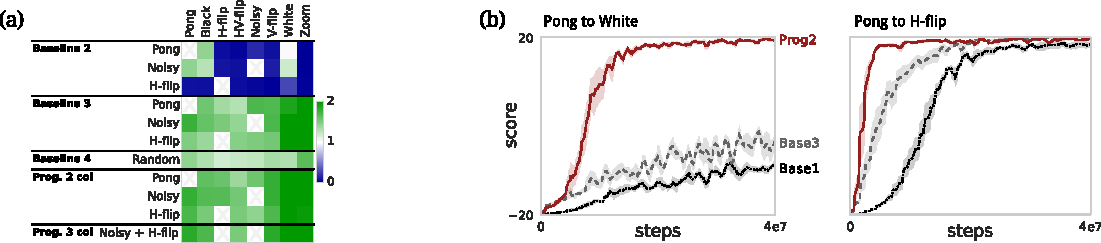
\includegraphics[width=1.\textwidth]{figures/transfer_pong.pdf}
    \caption{(a) Transfer matrix. Colours indicate transfer scores (clipped at 2).
      For progressive nets, the first column is trained on Pong, Noisy,
      or H-flip (table rows); the second column is trained on each of the
      other pong variants (table columns). (b) Example learning curves.}
    \label{fig:atari_results}
    \label{pong_results}
\end{figure}

We can make
several observations from these results. Baseline 2 (single column, only output layer is finetuned; see Fig.~\ref{fig:baselines})
fails to learn the target task in most
experiments and thus has negative transfer. This approach is quite standard
in supervised learning settings, where features from
ImageNet-trained nets are routinely repurposed for new domains.
As expected, we observe high positive transfer with baseline 3 (single column, full finetuning),
a well established paradigm for transfer.
Progressive networks outperform this baseline however in terms of both median and mean score, with
the difference being more pronounced for the latter. As the mean is
more sensitive to outliers, this suggests that progressive networks are better
able to exploit transfer when transfer is possible (i.e. when source and target domains are compatible). Fig.~\ref{pong_results}~(b) lends
weight to this hypothesis, where progressive networks are shown to significantly
outperform the baselines for particular game pairs.
Progressive nets also compare
favourably to baseline 4,
confirming that progressive nets are indeed taking
advantage of the features learned in previous columns.

\textbf{Detailed analysis}

\begin{figure}[h]
  \centering
    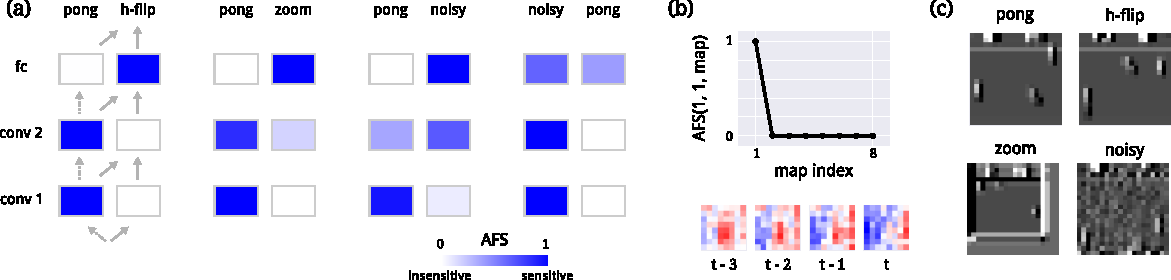
\includegraphics[width=.95\textwidth]{figures/pong_results_neil.pdf}
    \caption{(a) Transfer analysis for 2-column nets on Pong variants.
      The relative sensitivity of the network's outputs on the columns
      within each layer (the AFS) is indicated by the darkness of shading.
      (b) AFS values for the 8 feature maps of
      conv. 1 of a 1-column Pong net. Only one feature map is
      effectively used by the net; the same map is also used by the
      2-column versions. Below: spatial filter components (red =
      positive, blue = negative). (c) Activation maps of the filter in (b) from example
      states of the four games.}
    \label{fig:pong_results_neil}
\end{figure}

We use the metric derived in Sec.~\ref{sec_transfer} to
analyse what features are being transferred between Pong variants.
We see that when switching from Pong to H-Flip, the network reuses the
same components of low and mid-level vision (the outputs of the two
convolutional layers; Figure \ref{fig:pong_results_neil}a). However, the fully connected layer must be
largely re-learned, as the policy relevant features of the task (the
relative locations/velocities of the paddle and ball) are now in a new
location. When switching from Pong to Zoom, on the other hand,
low-level vision is reused for the new task, but new mid-level vision
features are learned. Interestingly, only one low-level feature appears
to be reused:
(see Fig.~\ref{fig:pong_results_neil}b): this is a spatio-temporal
filter with a considerable temporal DC component. This appears
sufficient for detecting both ball motion and paddle position in the
original, flipped, and zoomed Pongs.

Finally, when switching from Pong to Noisy, some new low-level
vision is relearned. This is likely because the first layer
filter learned on the clean task is not sufficiently
tolerant to the added noise. In contrast, this problem does not apply
when moving from Noisy to Pong (Figure
\ref{fig:pong_results_neil}a, rightmost column), where all of vision
transfers to the new task.


\subsection{Atari Games}

We next investigate feature transfer between randomly
selected Atari games~\cite{bellemare13arcade}. This is an interesting question, because the visuals of
Atari games are quite different from each other, as are the controls
and required strategy. Though games like Pong and Breakout are
conceptually similar (both involve hitting a ball with a
paddle), Pong is vertically aligned while
Breakout is horizontal: a potentially insurmountable
feature-level difference. Other Atari game pairs have \emph{no} discernible
overlap, even at a conceptual level.

\begin{figure}[h]
  \centering
    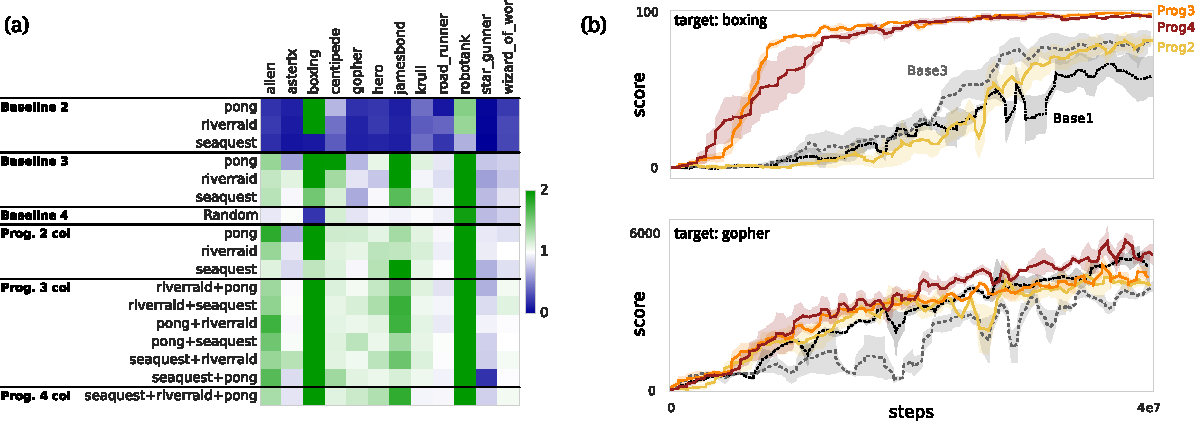
\includegraphics[width=.95\textwidth]{figures/transfer_atari.pdf}
    \caption{Transfer scores and example learning curves for Atari target games,
      as per Figure \ref{pong_results}.}
    \label{fig:atari_results}
\end{figure}

To this end we start by training single columns on three \emph{source}
games (Pong, River Raid, and Seaquest)
\footnote{Progressive columns having more than one ``source'' column are trained
sequentially on these source games, i.e.\ Seaquest-River Raid-Pong means column 1 is first trained
on Seaquest, column 2 is added afterwards and trained on River Raid, and then column 3 added and
trained on Pong.}
and assess if the learned features transfer to a different subset of
randomly selected \emph{target} games (Alien, Asterix, Boxing, Centipede,
Gopher, Hero, James Bond, Krull, Robotank, Road Runner, Star Gunner,
and Wizard of Wor). We evaluate progressive networks with 2, 3 and 4
columns, comparing to the baselines of Figure \ref{fig:baselines}).
The transfer matrix and selected transfer curves are shown in
Figure~\ref{fig:atari_results}, and the results summarized in
Table~\ref{table:main}.

Across all games, we observe from Fig.~\ref{fig:atari_results},
that progressive nets result in
positive transfer in 8 out of 12 target tasks, with only two cases
of negative transfer. This compares favourably to baseline 3, which yields
positive transfer in only 5 of 12 games. This trend is reflected in
Table~\ref{table:main}, where progressive networks convincingly outperform
baseline 3 when using additional columns. This is especially promising as
we show in the Appendix that progressive network use a diminishing amount of
capacity with each added column, pointing a clear path to online compression
or pruning as a means to mitigate the growth in model size.

Now consider the specific sequence
\textit{Seaquest}-to-\textit{Gopher}, an example of two dissimilar games. Here, the
pretrain/finetune paradigm (baseline 3) exhibits negative transfer, unlike
progressive networks (see Fig.\ref{fig:atari_results}b, bottom), perhaps
because they are more able to ignore the irrelevant features. For the sequence
\textit{Seaquest[+River Raid][+Pong]}-to-\textit{Boxing}, using additional
columns in the progressive networks can yield a significant increase in
transfer (see Fig.~\ref{fig:atari_results}b, top).

\begin{table}[t]
\begin{center}
\small
\begin{tabular}{@{}lrrrrrr@{}}
 \toprule
& \multicolumn{2}{c}{\textbf{Pong Soup}}
& \multicolumn{2}{c}{\textbf{Atari}}
& \multicolumn{2}{c}{\textbf{Labyrinth}}\\
                    & Mean (\%)    & Median (\%)  & Mean (\%)    & Median (\%)  & Mean (\%)     & Median (\%)  \\
 \midrule
  Baseline 1        & 100          & 100          & 100          & 100          & 100           & 100          \\
  Baseline 2        & 35           & 7            & 41           & 21           & 88            & 85           \\
  Baseline 3        & 181          & 160          & 133          & 110          & 235           & 112          \\
  Baseline 4        & 134          & 131          & 96           & 95           & 185           & 108          \\
  Progressive 2 col & 209          & 169          & 132          & 112          & \textbf{491}  & \textbf{115} \\
  Progressive 3 col & \textbf{222} & \textbf{183} & 140          & 111          & ---           & ---          \\
  Progressive 4 col & ---          & ---          & \textbf{141} & \textbf{116} & ---           & ---          \\

 \bottomrule
\end{tabular}
\end{center}
\caption{Transfer percentages in three domains. Baselines are defined in
    Fig.~\ref{fig:baselines}.}
\label{table:main}
\end{table}


\textbf{Detailed Analysis}

Figure \ref{fig:atari_results} demonstrates that both positive and
negative transfer is possible with progressive nets. To differentiate
these cases, we consider the Average Fisher Sensitivity for the 3 column
case (e.g., see Fig.~\ref{fig:atari3_results_neil}a). A clear pattern
emerges amongst these and other examples: the most negative transfer
coincides with complete dependence on the convolutional layers of the
previous columns, and no learning of new visual features in the new
column. In contrast, the most positive transfer occurs when the
features of the first two columns are \textit{augmented} by
new features. The statistics across all 3-column nets
(Figure \ref{fig:atari3_results_neil}b) show that positive transfer in
Atari occurs at a "sweet spot" between heavy reliance on features from
the source task, and heavy reliance on all new features for the
target task.

\begin{figure}[h]
  \centering 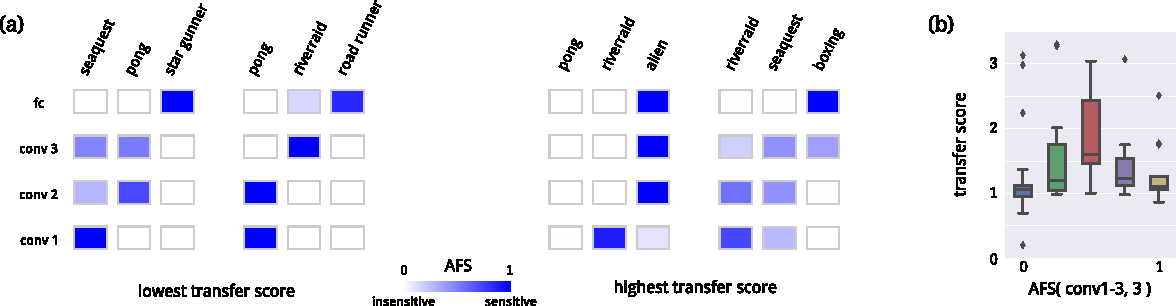
\includegraphics[width=.95\textwidth]{figures/atari3_results_neil.pdf} \caption{(a)
    AFS scores for 3-column nets with lowest (left) and highest
    (right) transfer scores on the 12 target Atari games. (b) Transfer
    statistics across 72 three-column nets, as a function of the
    mean AFS across the three convolutional layers of the new
    column (i.e.\ how much new vision is learned). } \label{fig:atari3_results_neil}
\end{figure}

At first glance, this result appears unintuitive: if a progressive net
finds a valuable feature set from a source task,
shouldn't we expect a high degree of transfer?
We offer two hypotheses. First, this may
simply reflect an optimization difficulty, where the source features offer
fast convergence to a poor local minimum. This is a known
challenge in transfer learning \cite{AAAIMag11-Taylor}: learned source
tasks confer an inductive bias that can either help or hinder in different cases.
Second, this may reflect a problem of
exploration, where the transfered representation is "good enough" for
a functional, but sub-optimal policy. 






\subsection{Labyrinth}

The final experimental setting for progressive networks is Labyrinth,
a 3D maze environment where the inputs are rendered images granting partial
observability and the agent outputs discrete actions,
including looking up, down, left, or right and moving forward,
backwards, left, or right. The tasks as well as the level maps are
diverse and involve getting positive scores for `eating' good items
(apples, strawberries) and negative scores for eating bad items
(mushrooms, lemons). Details can be found in the appendix. While there is conceptual and
visual overlap between the different tasks, the tasks present a
challenging set of diverse game elements (Figure
\ref{fig:datasets}).

\begin{figure}[h]
  \centering
    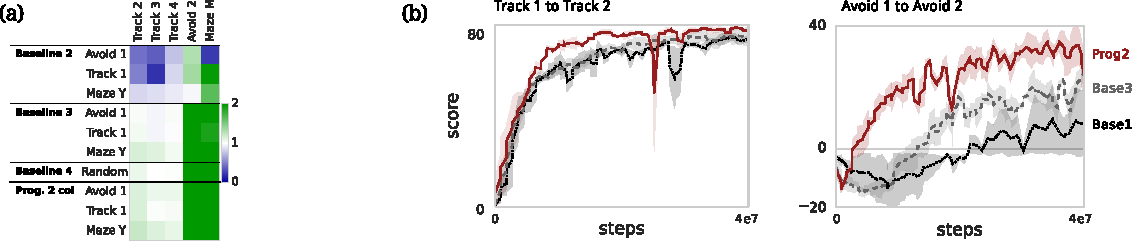
\includegraphics[width=\textwidth]{figures/transfer_lab.pdf}
    \caption{Transfer scores and example learning curves for Labyrinth tasks. Colours indicate transfer (clipped at 2). The learning curves show two examples of two-column progressive performance vs. baselines 1 and 3.}
    \label{fig:lab}
\end{figure}

As in the other domains, the progressive approach yields more positive transfer than any of the baselines (see Fig.~\ref{fig:lab}a and Table~\ref{table:main}). We observe less transfer on the Seek Track levels, which have dense reward items throughout the maze and are easily learned. Note that even for these easy cases, baseline 2 shows negative transfer because it cannot learn new low-level visual features, which are important because the reward items change from task to task. The learning curves in Fig.~\ref{fig:lab}b exemplify the typical results seen in this domain: on simpler games, such as Track 1 and 2, learning is rapid and stable by all agents. On more difficult games, with more complex game structure, the baselines struggle and progressive nets have an advantage.

\section{Discussion}
\label{discussion}

\subsection{DiffPD Simulation}
We conduct our simulation experiments based on a linear elastic corotated material setting. This energy model is popular for physical simulation and animation, but it is not the most accurate choice for closing the sim-to-real gap when deformations larger than about 200\% occur. This problem can be fixed by introducing a more sophisticated elastic energy model, for example a Neo-Hookean material.

\subsection{Experimental Setup}
Although the linear bearings in the experimental setup are well lubricated, they still contribute some friction. In the scope of this work, this friction force is assumed to be negligible. Furthermore, due to the rather small size of the tank, a standing wave persists in the tank even quite long after interacting with it. This can lead to a disturbance force on the load cell. However, since the frequency of this disturbance is known, it can be filtered out during post-processing.

% put in discussion about measurement dynamics

\subsection{Hydrodynamics}


% \subsection{Future Work}


\newpage
\footnotesize
\setlength{\bibsep}{5pt}
\bibliographystyle{plain}
\bibliography{progressive}

\newpage

\appendix
\pagenumbering{arabic}

{\Large{\textbf{Supplementary Material}}}

\section{Perturbation Analysis}

We explored two related methods for analysing transfer in progressive networks.
One based on Fisher information yields the Average Fisher Sensitivity (AFS)
and is described in Section 3 of the paper. We describe
the second method based on perturbation analysis in this appendix, as it proved
too slow to use at scale. Given its intuitive appeal however, we provide
details of the method along with results on Pong Variants (see
Section 5.2), as a means to corroborate the AFS score.

Our perturbation analysis aims to estimate which components of the source
columns materially contribute to the performance of the final column on the
target tasks. To this end, we injected Gaussian noise into each of the (post-ReLU) hidden
representations, with a new sample on every forward pass, and calculated the
average effect of these perturbations on the game score over 10 episodes.  We
did this at a coarse scale, by adding noise across all features of a given
layer, though a fine scale analysis is also possible per feature (map).
In order to be invariant to any arbitrary scale factors in the network weights,
we scale the noise variance proportional to the variance of the activations in
each feature map and fully-connected neuron. Scaling the variance in this
manner is analogous to computing the Fisher w.r.t. normalized activations for
the AFS score.

\begin{figure}[h]
  \centering
    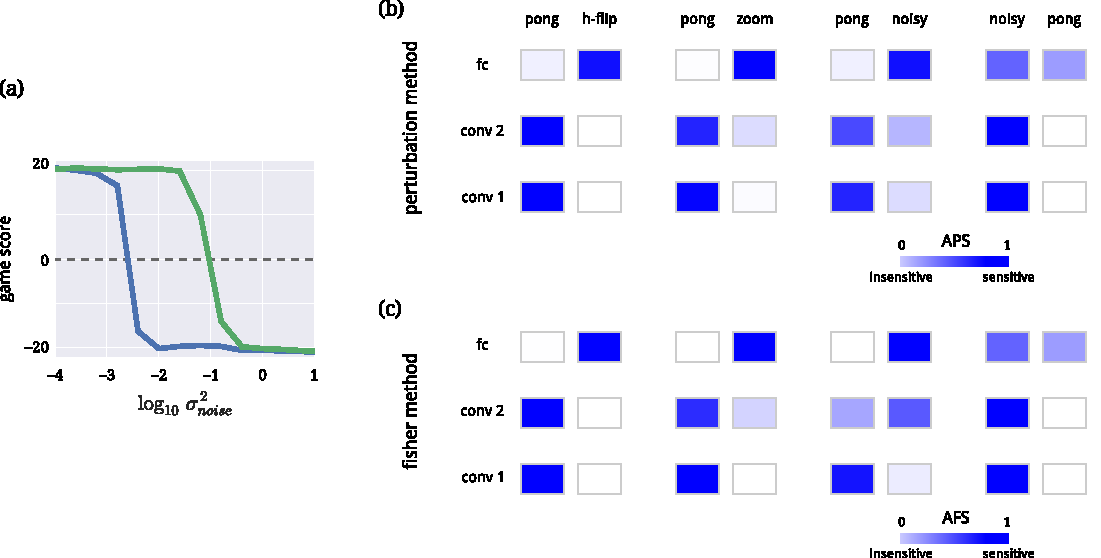
\includegraphics[width=.95\textwidth]{figures/appendix_AFS_vs_APS.pdf}
    \caption{(a) Perturbation analysis for the two second-layer
      convolutional representations in the two columns of the
      Pong/Pong-noise net. Blue: adding noise to second convolutional layer from column 1;
      green: from column 2. Grey line determines critical noise
      magnitude for each representation, $\sigma_i^2$.
      (b-c) Comparison of per-layer sensitivities obtained using the APS
      method (b) and the AFS method (c; as per main text).
      These are highly similar.}
    \label{fig:app_afs_vs_aps}
\end{figure}

Define ${\Lambda_i^{(k)}}=1/\sigma_i^{2(k)}$ as the precision of the noise
injected at layer $i$ of column $k$, which results in a $50\%$ drop in
performance. The Average Perturbation Sensitivity (APS) for this layer is
simply:
\begin{align}
    \text{APS}(i,k) = \frac{\Lambda_i^{(k)}}{\sum_k \Lambda_i^{(k)}}
\end{align}
Note that this value is normalized across columns for a given layer. The APS
score can thus be interpreted as the responsibility of each column in a given
layer to final performance.
The APS score of 2-column progressive networks trained on Pong Variants is
shown in Fig\ref{fig:app_afs_vs_aps} (b). These clearly corroborate the
AFS shown in (c).

\section{Compressibility of Progressive Networks}

As described in the main text, one of the limitations of progressive networks is the growth in the size of the network with added tasks. In the basic approach we pursue in the main text, the number of hidden units and feature maps grows linearly with the number of columns, and the number of parameters grows quadratically.

Here, we sought to determine the degree to which this full capacity is actually used by the network. We leveraged the Average Fisher Sensitivity measure to study how increasing the number of columns in the Atari task set changes the need for additional resources. In Figure \ref{fig:app_compression}a, we measure the average fractional use of \textit{existing} feature maps in a given layer (here, layer 2). We do this for each network by concatenating the per-feature-map AFS values from all source columns in this layer, sorting the values to produce a spectrum, and then averaging across networks. We find that as the number of columns increases, the average spectrum becomes sparser: the network relies on a smaller proportion of features from the source columns. Similar results were found for all layers. 

Similarly, in Figure \ref{fig:app_compression}b, we measure the capacity required in the final added column as a function of the total number of columns. Again, we measure the spectrum of AFS values in an example layer, but here from only the final column. As the progressive network grows, the new column's features are both less important overall (indicated by the declining area under the graph), and have a sparser AFS spectrum. Combined, these results suggest that significant pruning of lateral connections is possible, and the quadratic growth of parameters might be contained.

\begin{figure}[h]
  \centering
    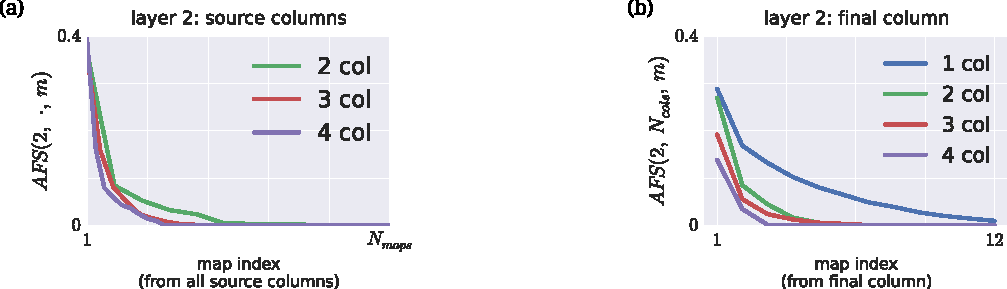
\includegraphics[width=.95\textwidth]{figures/appendix_compression.pdf}
    \caption{(a) Spectra of AFS values (for layer 2) across all feature maps from source columns, for the Atari dataset. The spectra show the range of AFS values, and are averaged across networks. While the 2 column / 3 column / 4 column nets all have different values of $N_{maps}$ (here, 12, 24, and 36 respectively), these have been dilated to fit the same axis to show the proportional use of these maps. (b) Spectra of AFS values (for layer 2) for the feature maps from only the final column. 
      }
    \label{fig:app_compression}
\end{figure}


\section{Setup Details}
\label{sec:appendix_jobs_detail}

In our grid we sample hyper-parameters from categorical distributions:
\begin{itemize}
  \item Learning rate was sampled from $\{10^{-3}, 5\cdot 10^{-4}, 10^{-4}\}$.
  \item Strength of the entropy regularization from $\{10^{-2}, 10^{-3}, 10^{-4}\}$
  \item Gradient clipping cut-off from $\{20, 40\}$
  \item scalar multiplier on the lateral feature is initialized randomly to one from $\{1, 10^{-1}, 10^{-2}\}$
\end{itemize}

For the Atari experiments we used a model with 3 convolutional layers followed by a fully connected
layer and from which we predict the policy and value function. The convolutional layers are as
follows. All have 12 feature maps. The first convolutional layer has a kernel of size 8x8 and a stride
of 4x4. The second layer has a kernel of size 4 and a stride of 2. The last convolutional layer has
size 3x4 with a stride of 1.  The fully connected layer has 256 hidden units.

Learning follows closely the paradigm described in \citep{mnih2016a3c}. We use 16 workers and the
same RMSProp algorithm without momentum or centring of the variance. The score for each point of
a training curve is the average over all the episodes the model gets to finish in $25e4$ environment steps.

The whole experiments are run for a maximum of $1.6e8$ environment step. The agent has an action repeat of 4 as
in \cite{mnih2016a3c}, which means that for 4 consecutive steps the agent will use the same action picked at the
beginning of the series. For this reason through out the paper we actually report results in terms of agent
perceived steps rather than environment steps. That is, the maximal number of agent perceived step that we do
for any particular run is $4e7$.

\section{Learning curves}
\label{sec:appendix_curves}

Figure \ref{fig:app_plot} shows training curves for all the \textit{target} games in the Atari domain.
We plot learning curves for two column, three column and four column progressive networks alongside Baseline 3 (gray dashed line), a model pretrained on Seaquest and then finetuned on the particular \textit{target} game and Baseline 1 (gray dotted line), where a single column is trained on the \textit{source} game Seaquest.

\begin{figure}
     \begin{tabular}{ccc}
        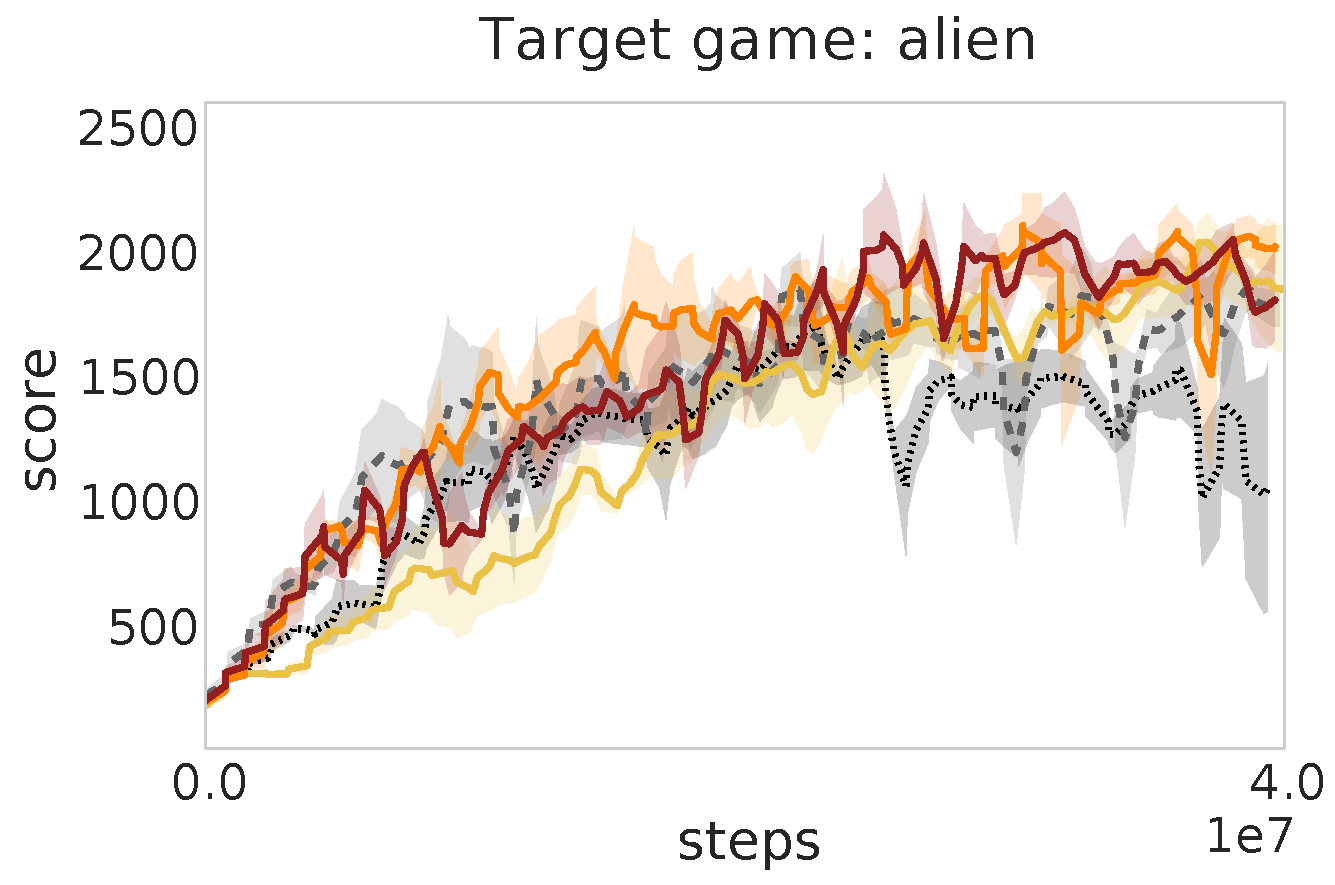
\includegraphics[width=.33\textwidth]{figures/app_plots/mainpaper-nolegend-seaquest_riverraid_pong_to_alien} &
        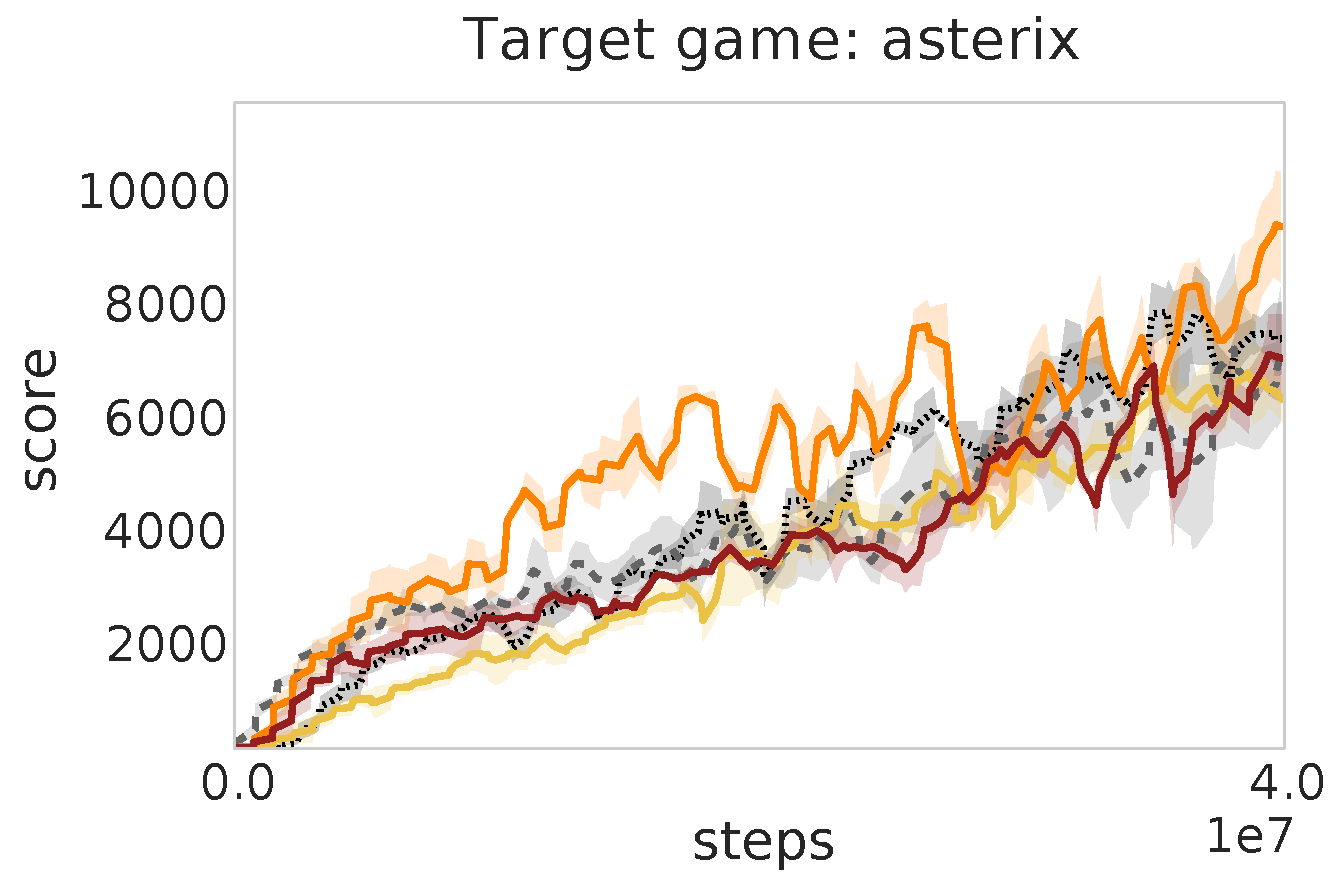
\includegraphics[width=.33\textwidth]{figures/app_plots/mainpaper-nolegend-seaquest_riverraid_pong_to_asterix} &
        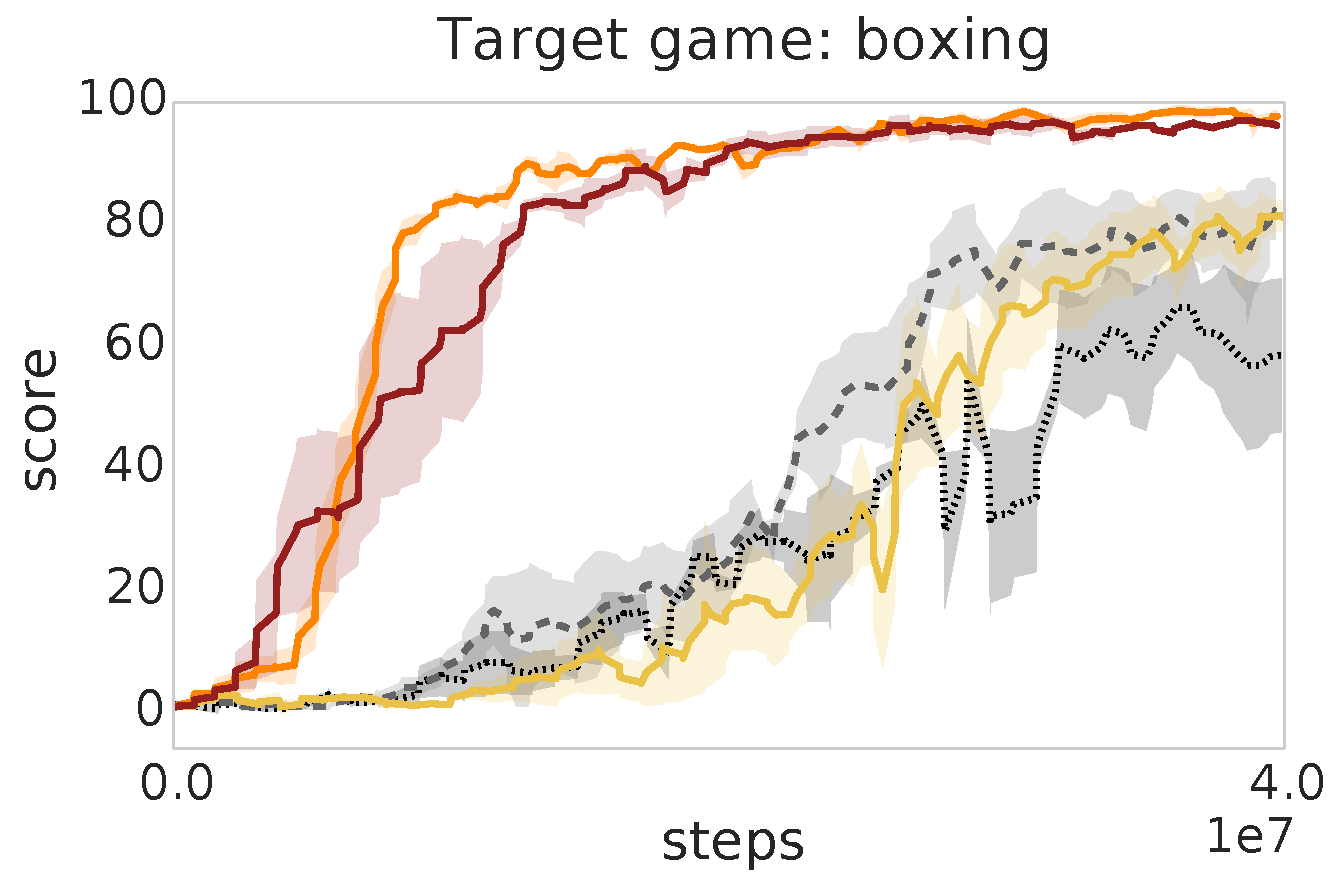
\includegraphics[width=.33\textwidth]{figures/app_plots/mainpaper-nolegend-seaquest_riverraid_pong_to_boxing} \\

        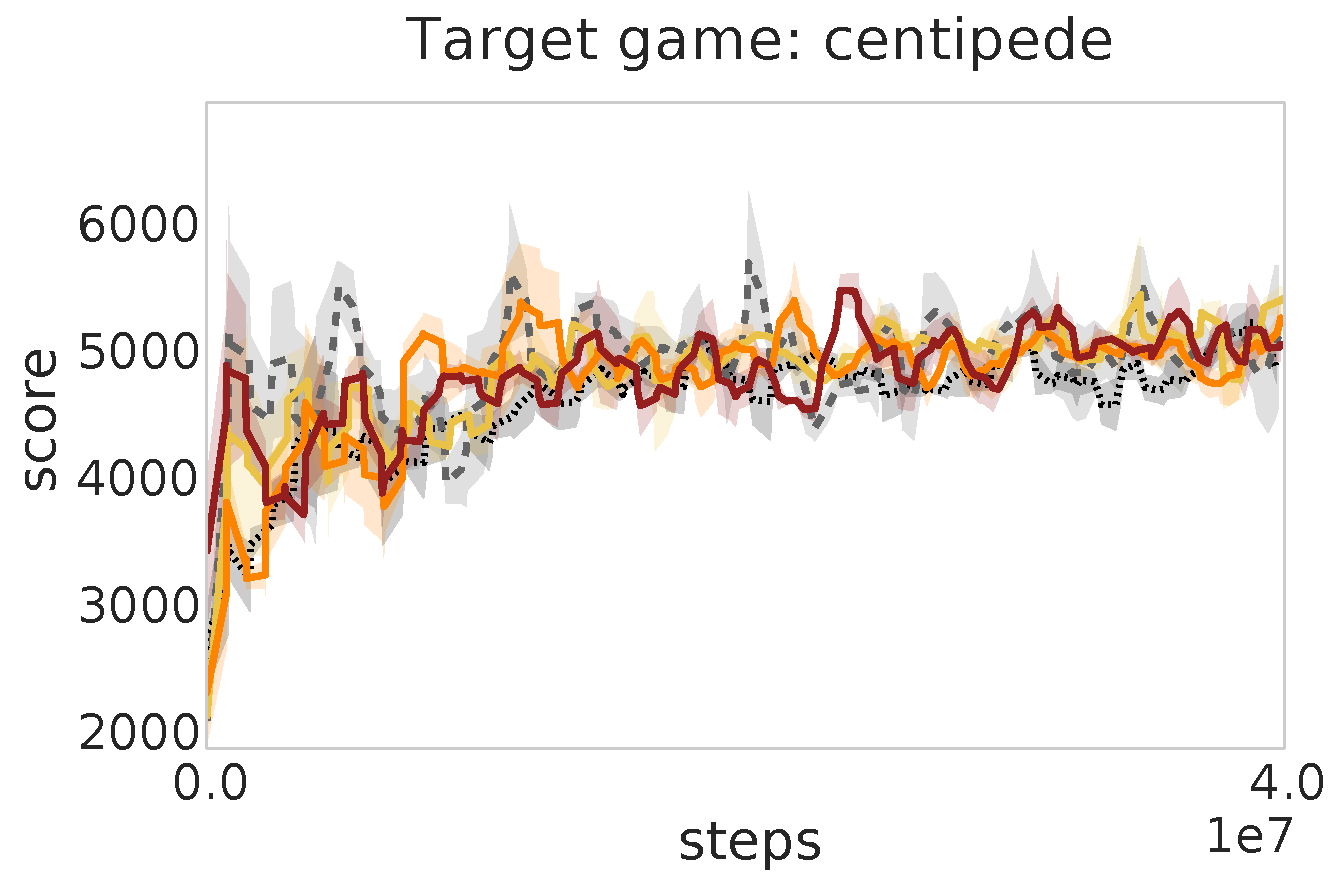
\includegraphics[width=.33\textwidth]{figures/app_plots/mainpaper-nolegend-seaquest_riverraid_pong_to_centipede} &
        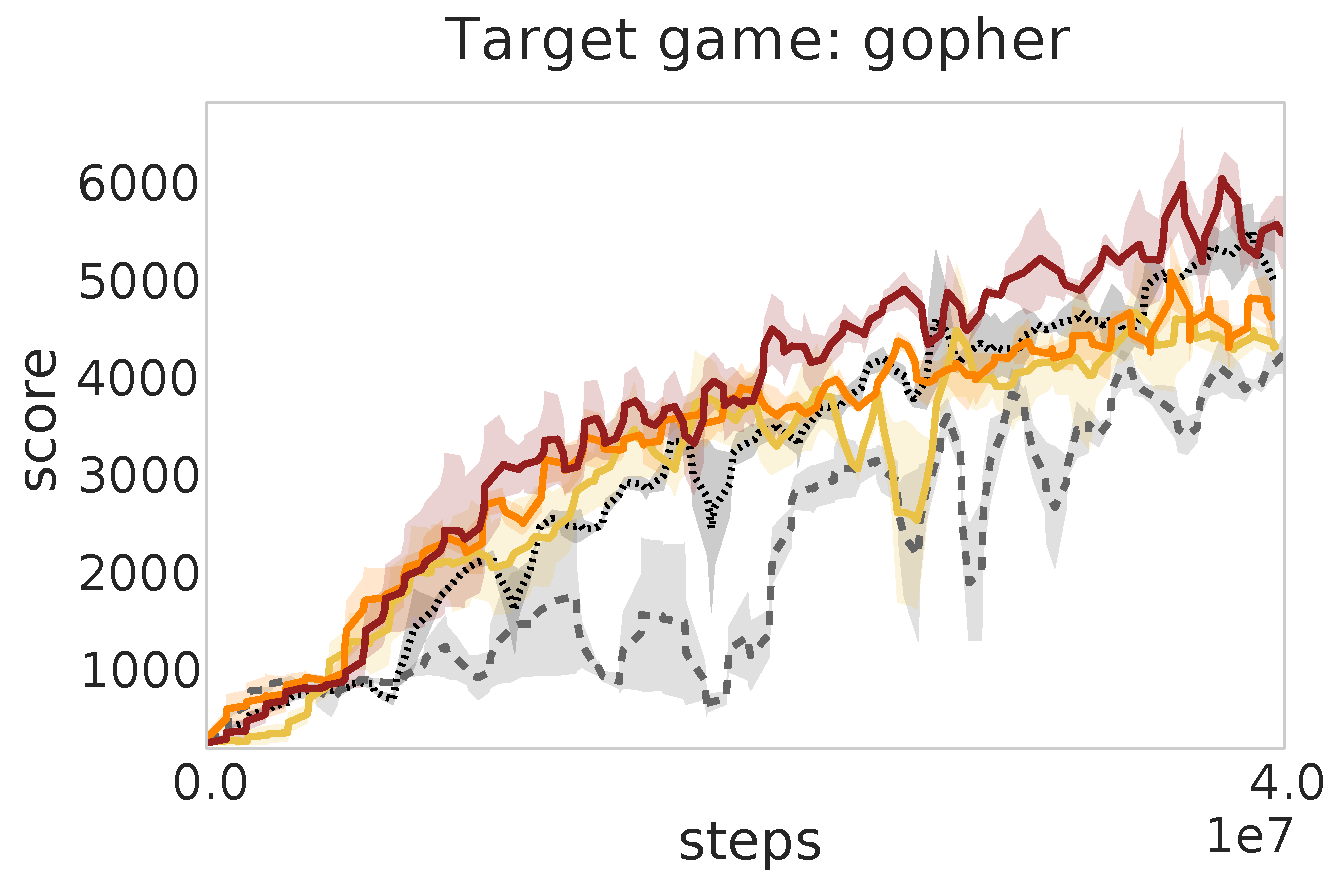
\includegraphics[width=.33\textwidth]{figures/app_plots/mainpaper-nolegend-seaquest_riverraid_pong_to_gopher} &
        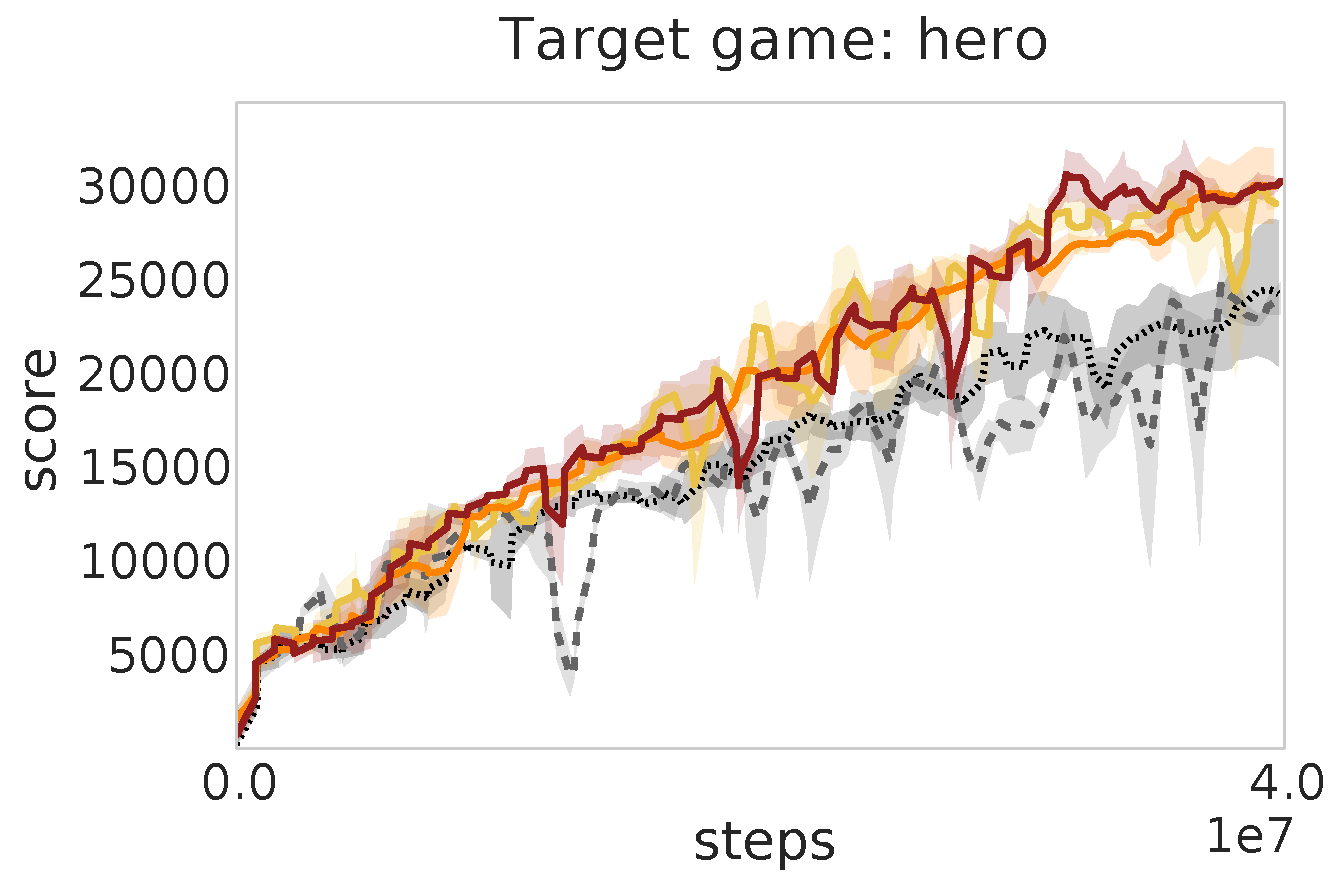
\includegraphics[width=.33\textwidth]{figures/app_plots/mainpaper-nolegend-seaquest_riverraid_pong_to_hero} \\

        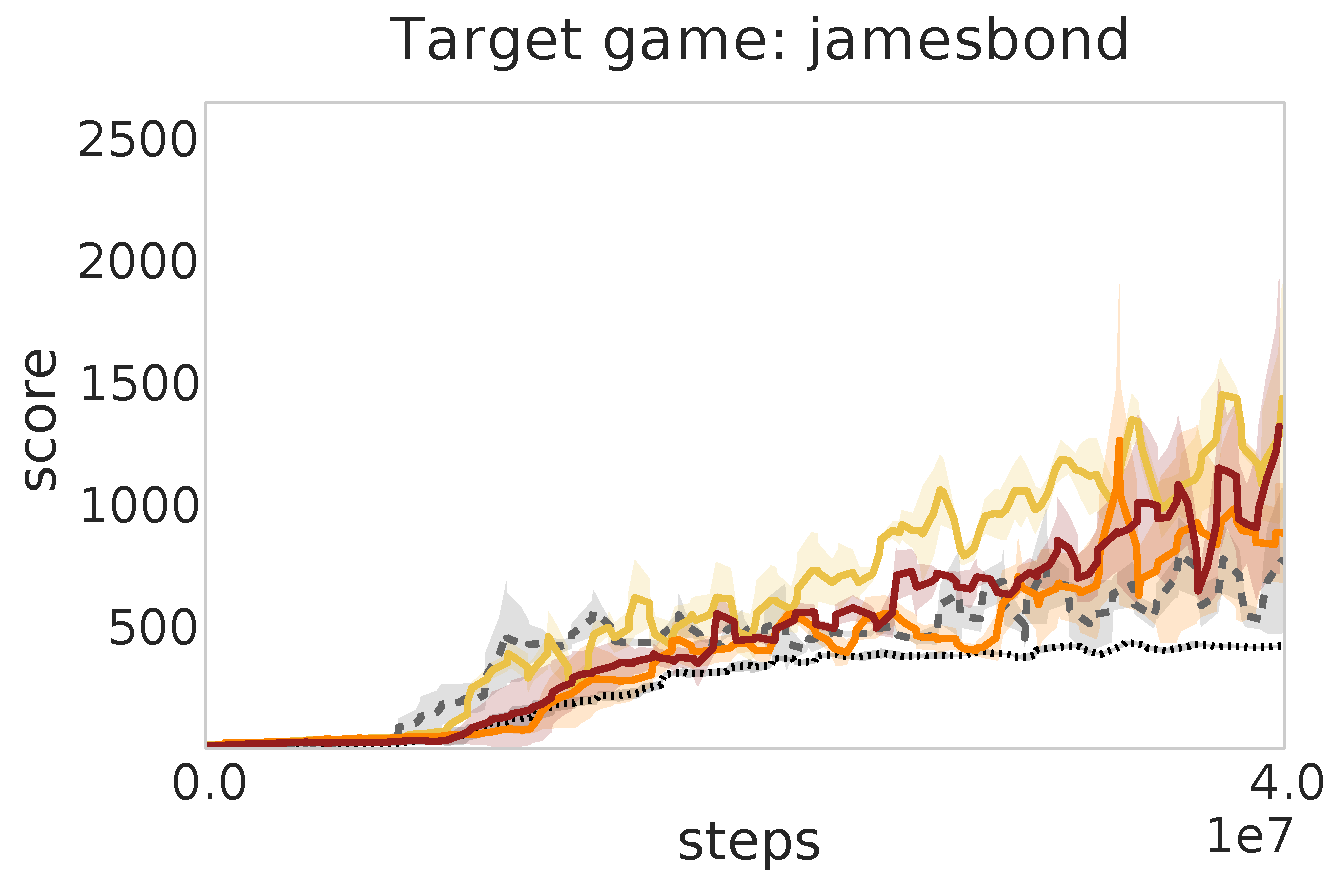
\includegraphics[width=.33\textwidth]{figures/app_plots/mainpaper-nolegend-seaquest_riverraid_pong_to_jamesbond} &
        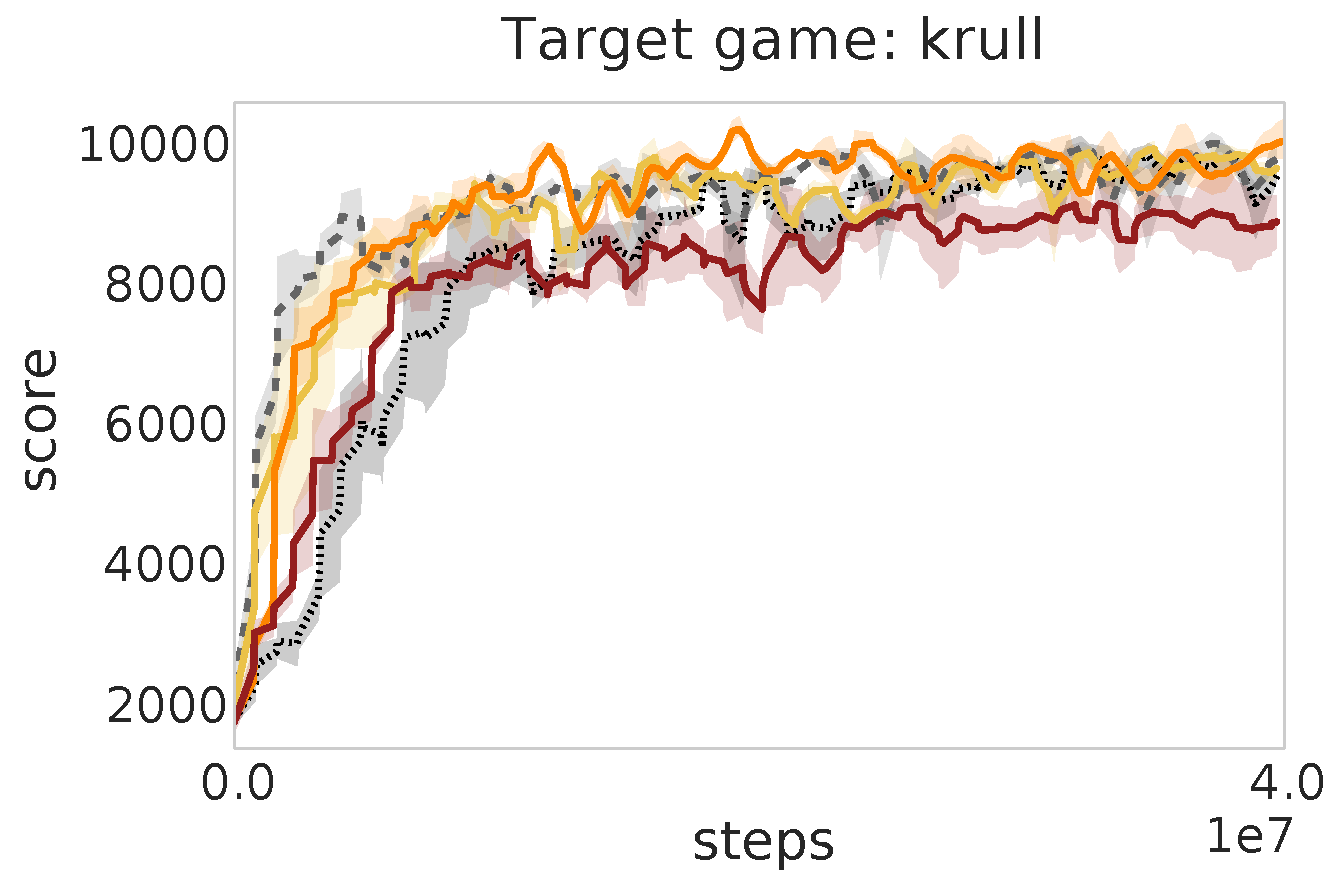
\includegraphics[width=.33\textwidth]{figures/app_plots/mainpaper-nolegend-seaquest_riverraid_pong_to_krull} &
        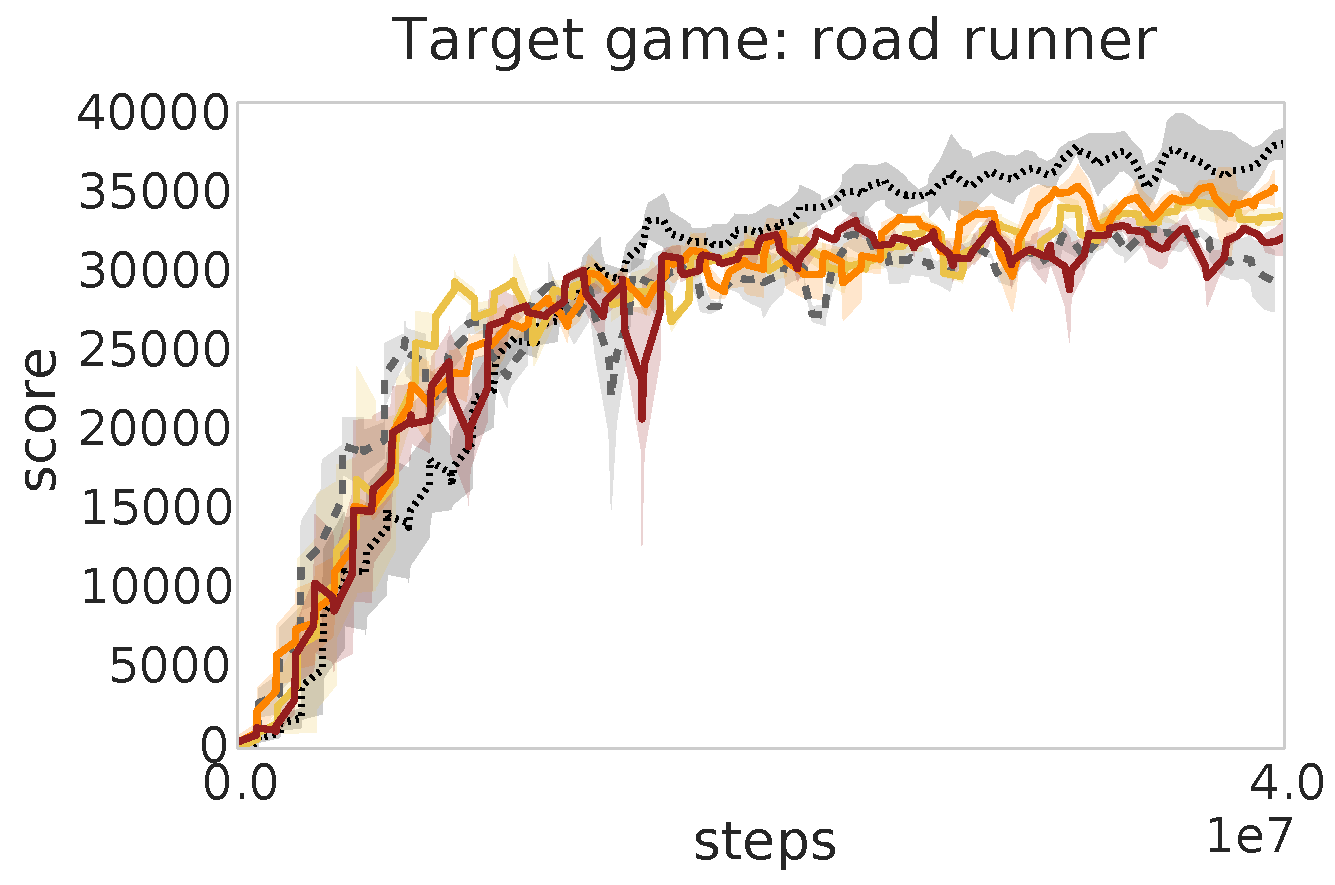
\includegraphics[width=.33\textwidth]{figures/app_plots/mainpaper-nolegend-seaquest_riverraid_pong_to_road_runner} \\

        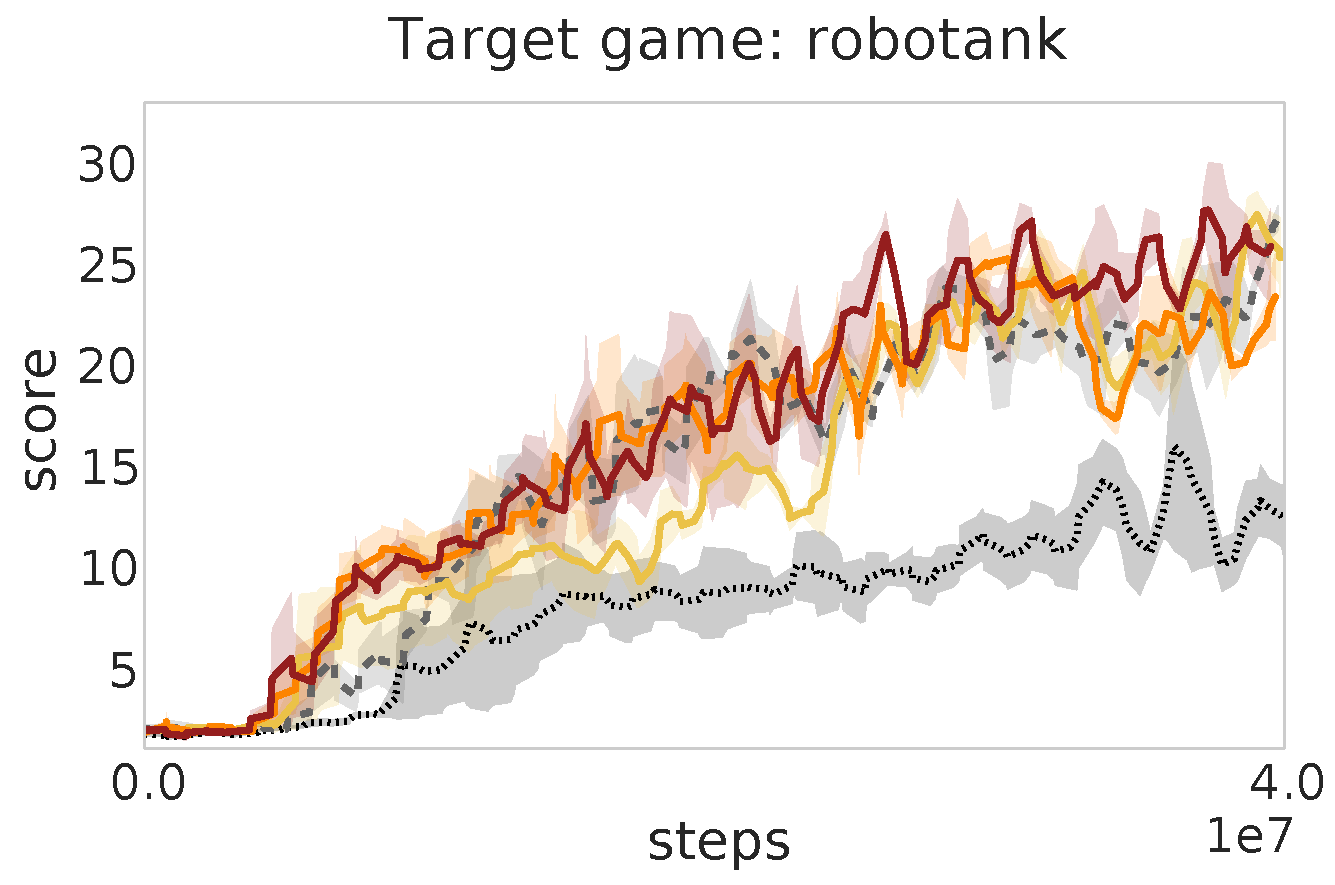
\includegraphics[width=.33\textwidth]{figures/app_plots/mainpaper-nolegend-seaquest_riverraid_pong_to_robotank} &
        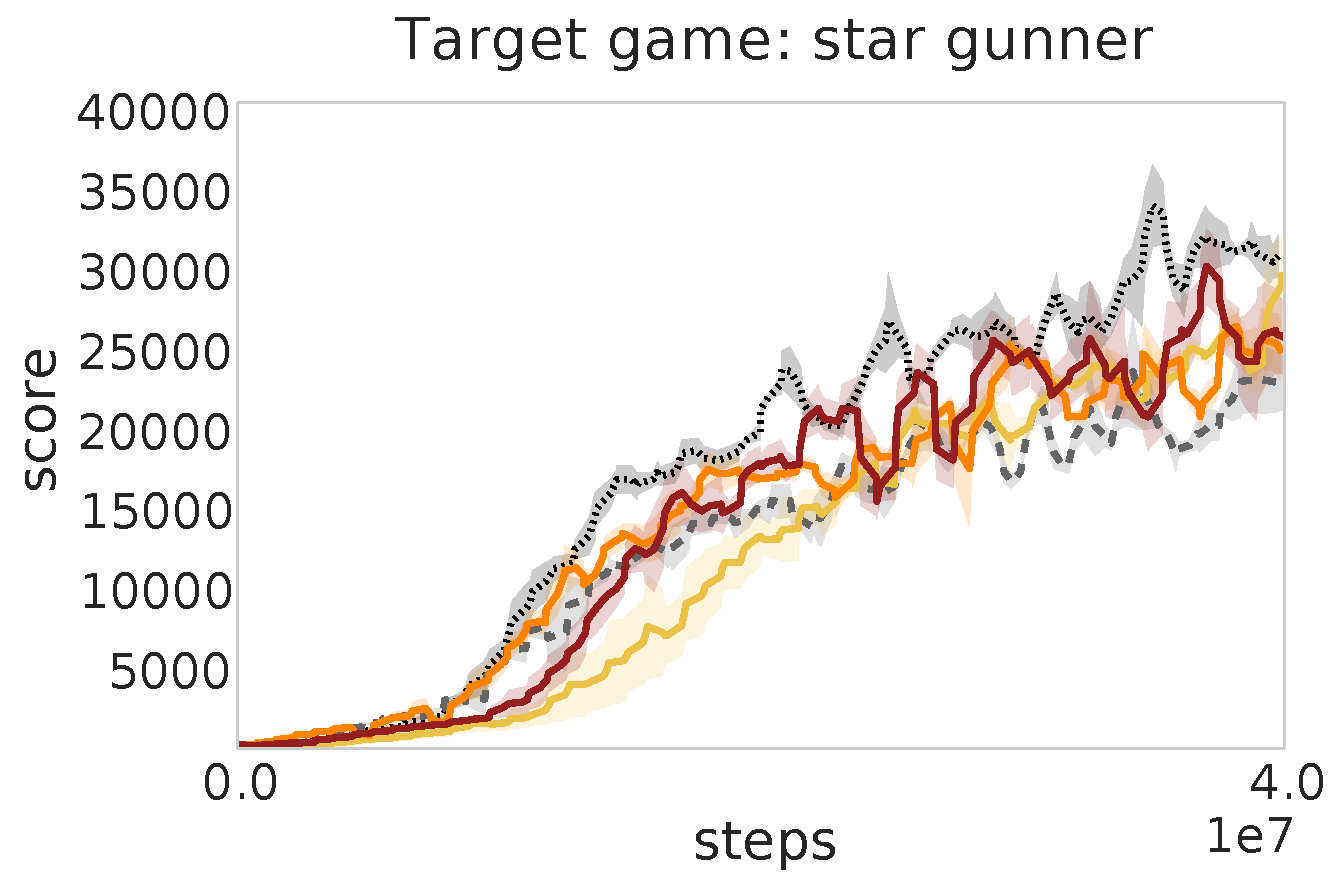
\includegraphics[width=.33\textwidth]{figures/app_plots/mainpaper-nolegend-seaquest_riverraid_pong_to_star_gunner} &
        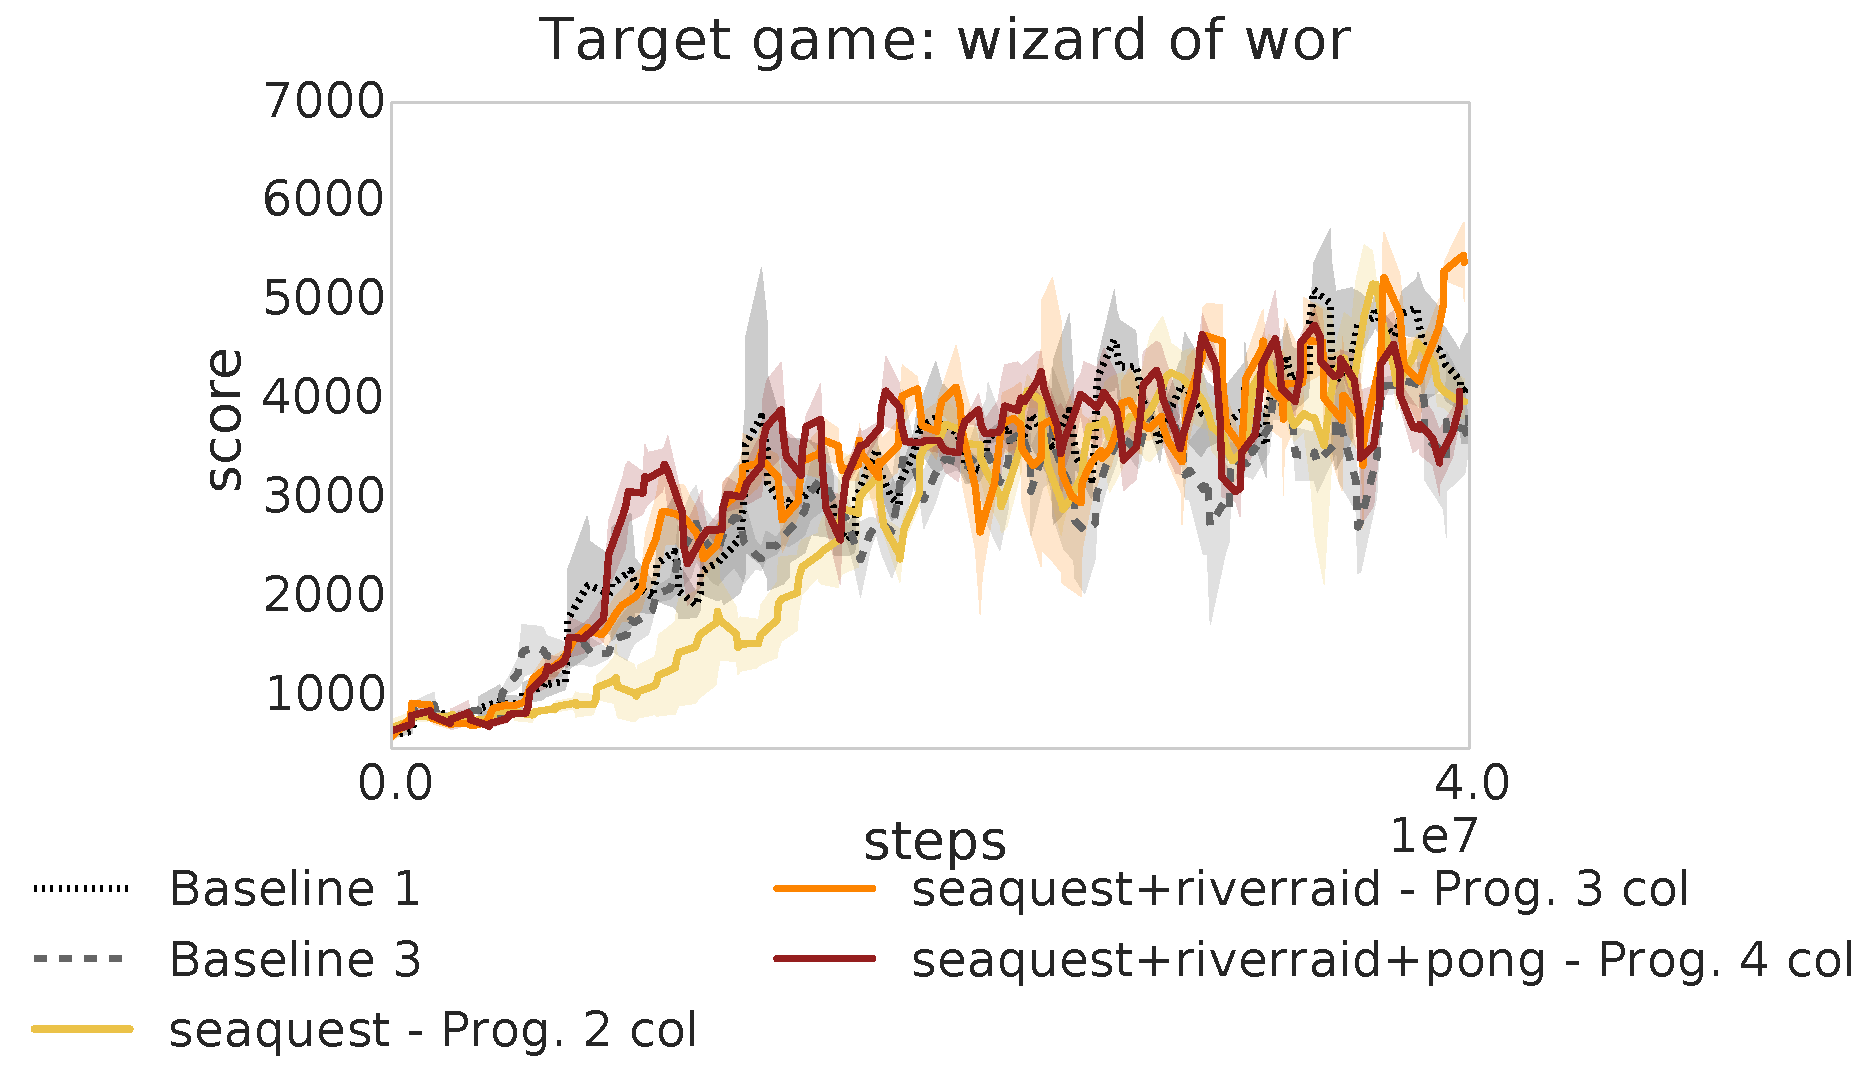
\includegraphics[width=.33\textwidth]{figures/app_plots/mainpaper-legend-seaquest_riverraid_pong_to_wizard_of_wor} \\
    \end{tabular}
    \caption{Training curves for transferring to the \textit{target} games after seeing first Seaquest followed by River Raid and lastly Pong. For the baselines,
    the \textit{source} game used for pretraining is Seaquest.}
    \label{fig:app_plot}
\end{figure}

We can see that overall baseline 3 performs well. However there are situations when having features learned from more previous task actually helps with transfer (e.g. when \textit{target} game is Boxing).

Figure \ref{fig:app_plot_pongs} shows how two-column progressive networks perform as compared to Baseline 3 (gray dashed line), a model pretrained on the \textit{source} game, here standard Pong, and then finetuned on a particular \textit{target} game, and Baseline 1 (black dotted line), where a single column is trained on standard Pong. Figure \ref{fig:app_plot_lab} shows two-column progressive networks and baselines on Labyrinth tasks; the \textit{source} game was Maze Y. 

\begin{figure}
     \begin{tabular}{cccccccc}
	Target: Pong & Target: Black \\
        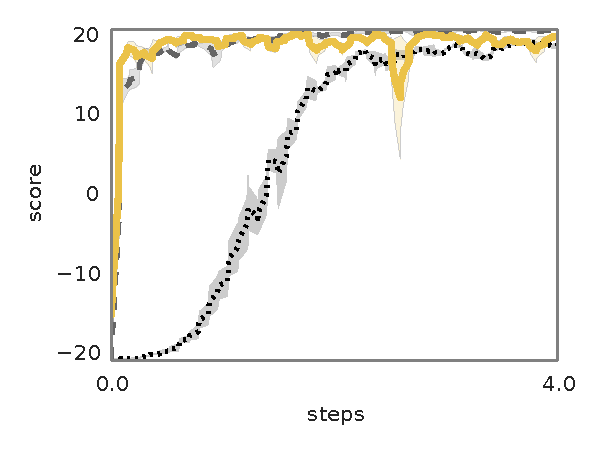
\includegraphics[width=.44\textwidth]{figures/app_plots/pongs/pong/pong} &
        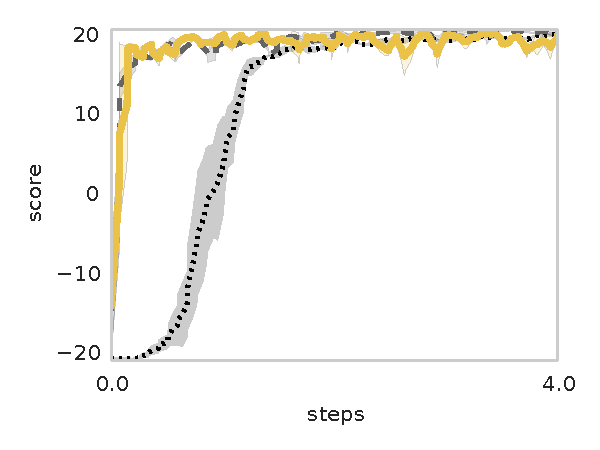
\includegraphics[width=.44\textwidth]{figures/app_plots/pongs/pong/pong_black} \\

	Target: H-flip & Target: HV-flip \\
        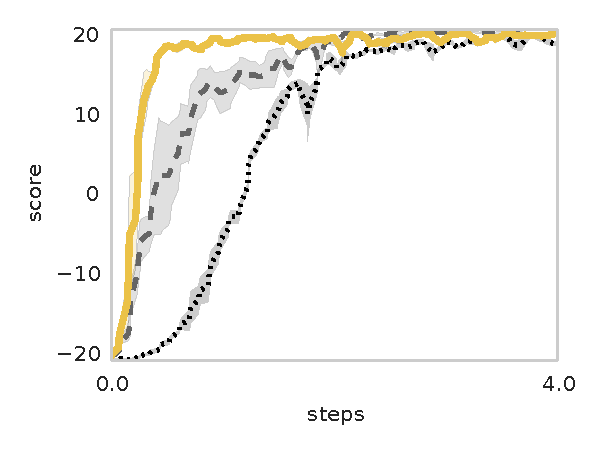
\includegraphics[width=.44\textwidth]{figures/app_plots/pongs/pong/pong_h_flip} &
        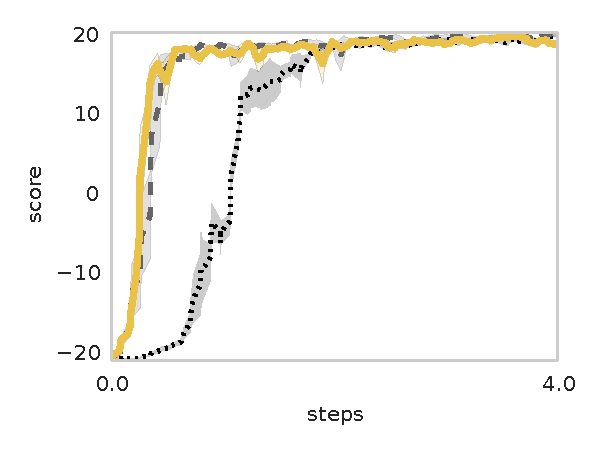
\includegraphics[width=.44\textwidth]{figures/app_plots/pongs/pong/pong_hv_flip} \\

	Target: Noisy & Target: V-flip \\
	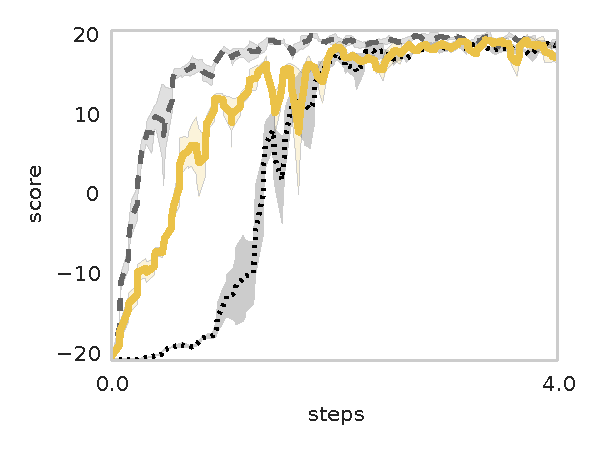
\includegraphics[width=.44\textwidth]{figures/app_plots/pongs/pong/pong_noise} &
        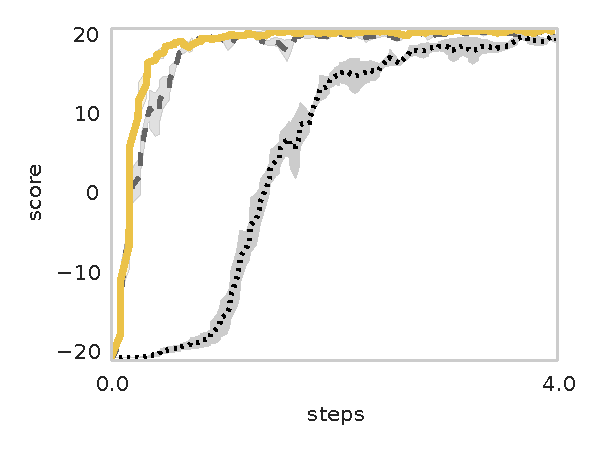
\includegraphics[width=.44\textwidth]{figures/app_plots/pongs/pong/pong_v_flip} \\

	Target: White & Target: Zoom \\
        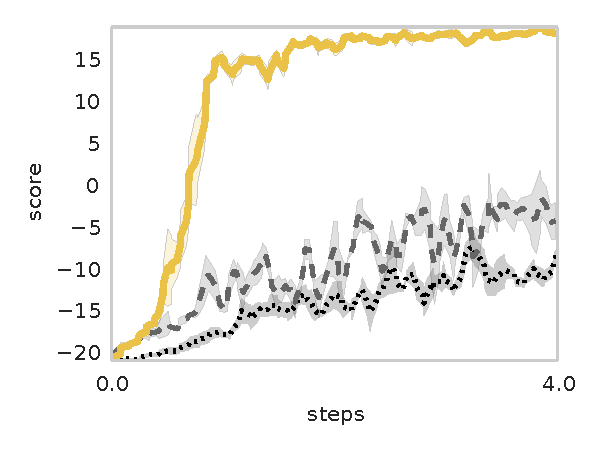
\includegraphics[width=.44\textwidth]{figures/app_plots/pongs/pong/pong_white} &
        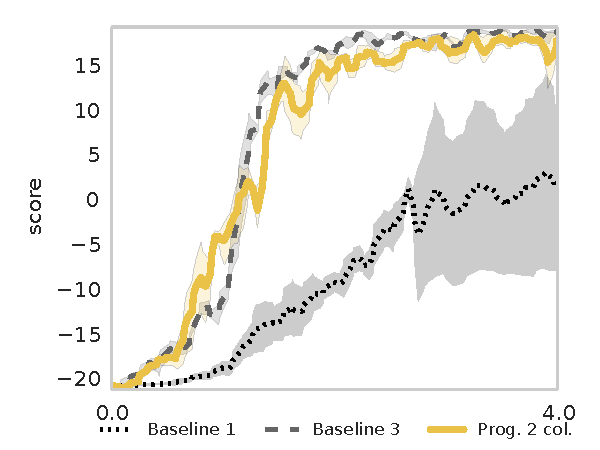
\includegraphics[width=.44\textwidth]{figures/app_plots/pongs_legend/pong/pong_zoom} \\

    \end{tabular}
\caption{Training curves for transferring to 8 \textit{target} games after learning standard Pong first. }
    \label{fig:app_plot_pongs}
\end{figure}

\begin{figure}
     \begin{tabular}{cccccccc}
	Target: Track 1 & Target: Track 2 \\
        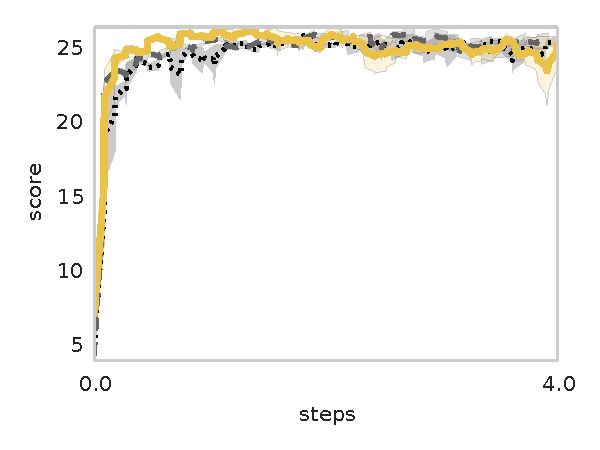
\includegraphics[width=.44\textwidth]{figures/app_plots/lab/smy1/seek_track_01} &
        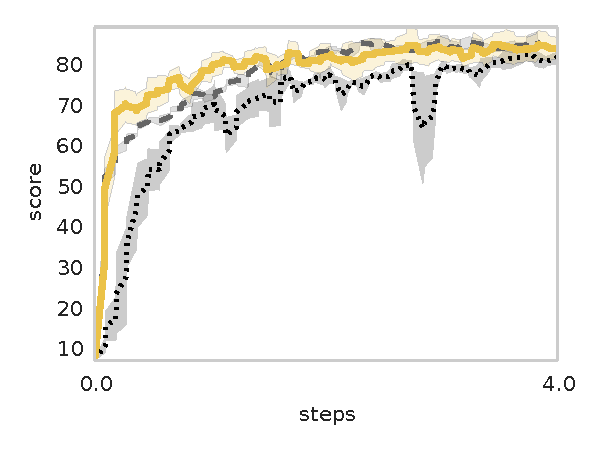
\includegraphics[width=.44\textwidth]{figures/app_plots/lab/smy1/seek_track_02} \\

	Target: Track 3 & Target: Track 4 \\
        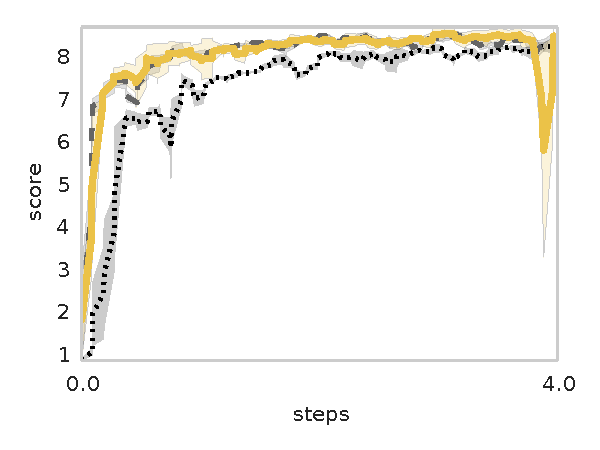
\includegraphics[width=.44\textwidth]{figures/app_plots/lab/smy1/seek_track_03} &
        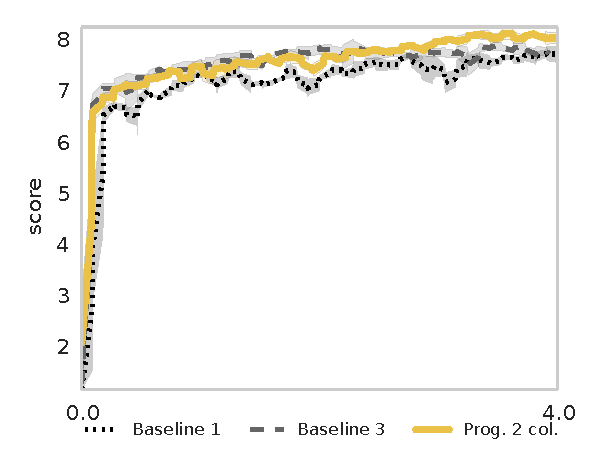
\includegraphics[width=.44\textwidth]{figures/app_plots/lab_legend/smy1/seek_track_04} \\

	Target: Avoid 1 & Target: Avoid 2 \\
        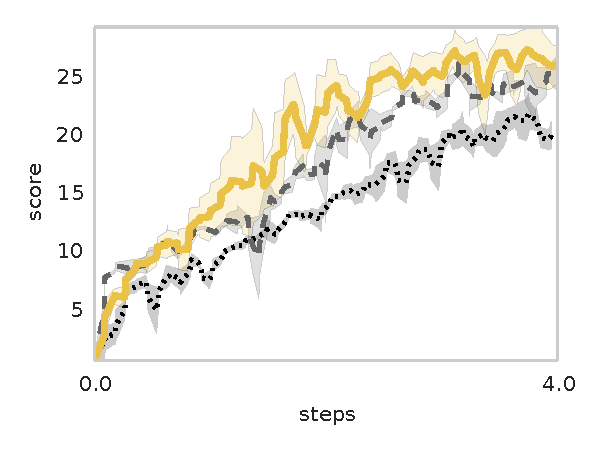
\includegraphics[width=.44\textwidth]{figures/app_plots/lab/smy1/seekavoid_arena_01} &
        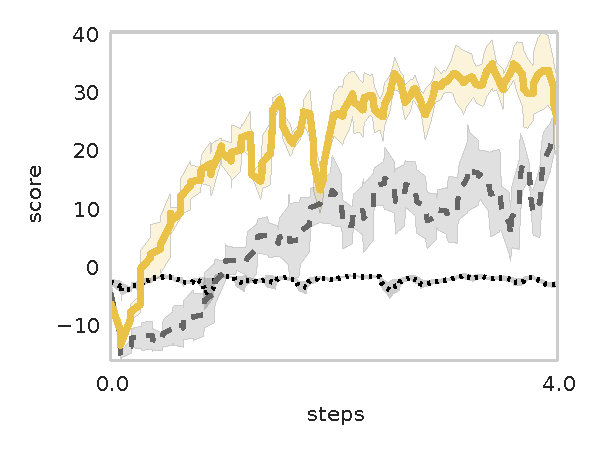
\includegraphics[width=.44\textwidth]{figures/app_plots/lab/smy1/seekavoid_arena_02} \\

	Target: Maze Y & Target: Maze M \\
        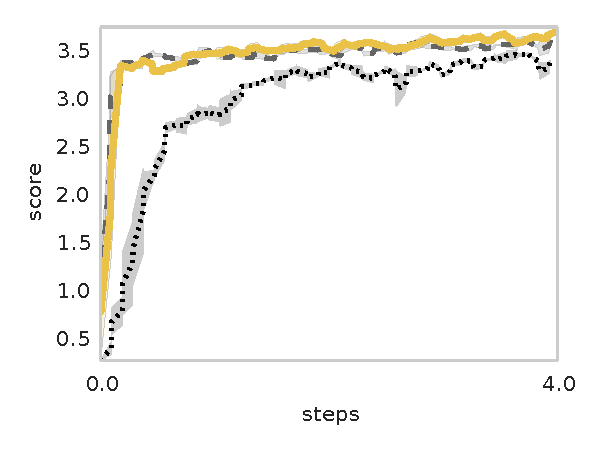
\includegraphics[width=.44\textwidth]{figures/app_plots/lab/smy1/seek_maze_y_01} &
        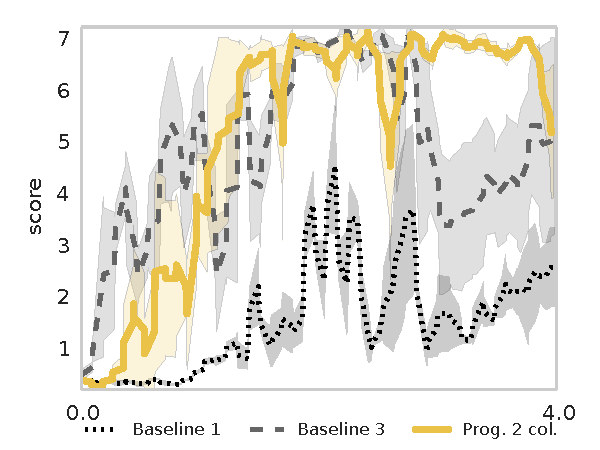
\includegraphics[width=.44\textwidth]{figures/app_plots/lab_legend/smy1/seek_maze_m_01} \\
    \end{tabular}
\caption{Training curves for transferring to 8 \textit{target} games after learning Maze Y first.}
    \label{fig:app_plot_lab}
\end{figure}


\section{Labyrinth}

Section 5.4 evaluates progressive networks on foraging tasks in complex 3D maze
environments. Positive rewards are given to the agent for collecting apples and
strawberries, and negative rewards for mushrooms and lemons.
Episodes terminate when either all (positive) rewards are collected, or after a
fixed time interval.

Levels differ in their maze layout, the type of items present and the sparsity
of the reward structure. The levels we employed can be characterized as follows:
\begin{itemize}
\item Seek Track 1: simple corridor with many apples
\item Seek Track 2: U-shaped corridor with many strawberries
\item Seek Track 3: $\Omega$-shaped, with $90^o$ turns, with few apples
\item Seek Track 4: $\Omega$-shaped, with $45^o$ turns, with few apples
\item Seek Avoid 1: large square room with apples and lemons
\item Seek Avoid 2: large square room with apples and mushrooms
\item Seek Maze M : M-shaped maze, with apples at dead-ends
\item Seek Maze Y : Y-shaped maze, with apples at dead-ends
\end{itemize}


\end{document}
